% =============================================================
% Harris + LK Object Tracking Report
% FAST NUCES — Spring 2026
% Ali Ahmad | 23L-2619
% =============================================================
\documentclass[12pt,a4paper]{article}

% --- Core packages -------------------------------------------
\usepackage[T1]{fontenc}
\usepackage[utf8]{inputenc}
\usepackage[a4paper, top=2.5cm, bottom=2.5cm, left=2.5cm, right=2.5cm, headheight=15pt]{geometry}
\usepackage{graphicx}
\usepackage{subcaption}
\usepackage{booktabs}
\usepackage{colortbl}
\usepackage{tabularx}
\usepackage{multirow}
\usepackage{amsmath}
\usepackage{amssymb}
\usepackage[dvipsnames]{xcolor}
\usepackage{fancyhdr}
\usepackage{titlesec}
\usepackage{tikz}
\usepackage{float}
\usepackage{parskip}
\usepackage{setspace}
\usepackage[protrusion=true,expansion=false]{microtype}
\usepackage{array}
\usepackage{enumitem}
\usepackage{makecell}
\usepackage{listings}
\usepackage[framemethod=TikZ]{mdframed}
\usepackage{tocloft}
\usepackage[backend=bibtex,style=numeric,sorting=none]{biblatex}
\addbibresource{refs.bib}

% Load hyperref AFTER tocloft and mdframed
\usepackage[colorlinks=true, linkcolor=accentteal, citecolor=accentteal, urlcolor=accentteal]{hyperref}

\usepackage{caption}

\usetikzlibrary{arrows.meta, shapes.geometric, positioning, fit, backgrounds}

% --- Color palette -------------------------------------------
\definecolor{reportblue}{HTML}{2E4057}
\definecolor{accentteal}{HTML}{1B6CA8}
\definecolor{darkbadge}{HTML}{2C3E50}
\definecolor{rulecolor}{HTML}{AAAAAA}

% --- Body text spacing ---------------------------------------
\setlength{\parskip}{4pt}
\setlength{\parindent}{0pt}
\linespread{1.05}

% --- Overflow tolerance --------------------------------------
\setlength{\emergencystretch}{5em}
\hfuzz=10pt

% --- Column types --------------------------------------------
\newcolumntype{R}{>{\raggedleft\arraybackslash}X}

% --- Caption formatting --------------------------------------
\captionsetup{font=small, labelfont={bf,color=accentteal}, labelsep=period}

% --- Section headings ----------------------------------------
\titleformat{\section}
  {\color{accentteal}\large\bfseries}
  {\thesection}{0.8em}{}
  [\vspace{2pt}\textcolor{rulecolor}{\titlerule[0.4pt]}]

\titlespacing*{\section}{0pt}{18pt plus 4pt minus 2pt}{8pt}

\titleformat{\subsection}
  {\color{accentteal}\normalsize\bfseries}
  {\thesubsection}{1em}{}

\titleformat{\subsubsection}
  {\color{accentteal}\normalsize\bfseries\itshape}
  {\thesubsubsection}{1em}{}

% Starred variants must be explicitly set
\titleformat*{\subsubsection}{\color{accentteal}\normalsize\bfseries\itshape}

% --- TOC styling (tocloft) -----------------------------------
\renewcommand{\cftsecfont}{\bfseries\color{accentteal}}
\renewcommand{\cftsubsecfont}{\color{accentteal}}
\renewcommand{\cftsecpagefont}{\bfseries}
\renewcommand{\cftsubsecpagefont}{}
\setlength{\cftbeforesecskip}{4pt}

% --- Running headers -----------------------------------------
\pagestyle{fancy}
\fancyhf{}
\fancyhead[L]{\small\textit{Harris + LK Object Tracking}}
\fancyhead[R]{\small\textit{FAST NUCES --- Spring 2026}}
\renewcommand{\headrulewidth}{0.4pt}
\fancyfoot[C]{\thepage}

% --- Listings ------------------------------------------------
\lstset{basicstyle=\small\ttfamily, frame=single,
        rulecolor=\color{accentteal}, framesep=4pt}

% --- Graphics path -------------------------------------------
\graphicspath{{imgs/}}

% ============================================================
\begin{document}
% ============================================================

% --- Cover page ---------------------------------------------
\begin{titlepage}
\thispagestyle{empty}

{\centering
  {\large\bfseries\color{reportblue}
    National University of Computer \& Emerging Sciences}\\[4pt]
  {\normalsize\color{reportblue} FAST NUCES --- Lahore Campus}\\[18pt]
  \noindent\textcolor{accentteal}{\rule{\linewidth}{2pt}}\\[-4pt]
  \noindent\textcolor{accentteal}{\rule{\linewidth}{0.4pt}}\\[14pt]
  {\small Department of Data Science \& Artificial Intelligence}\\[4pt]
  {\small Fundamentals of Computer Vision \quad --- \quad Spring 2026}\\[8pt]
  \noindent\textcolor{rulecolor}{\rule{\linewidth}{0.4pt}}
\par}

\vspace{3cm}

\begin{mdframed}[
  linecolor=accentteal,
  linewidth=1.2pt,
  roundcorner=8pt,
  innertopmargin=14pt,
  innerbottommargin=14pt,
  innerleftmargin=20pt,
  innerrightmargin=20pt,
  backgroundcolor=white
]
  \centering
  {\Large\bfseries\color{accentteal}
    Feature-Based Object Tracking using Harris Corners\\[4pt]
    and Lucas--Kanade Optical Flow}
\end{mdframed}

\vspace{1.5cm}

\begin{center}
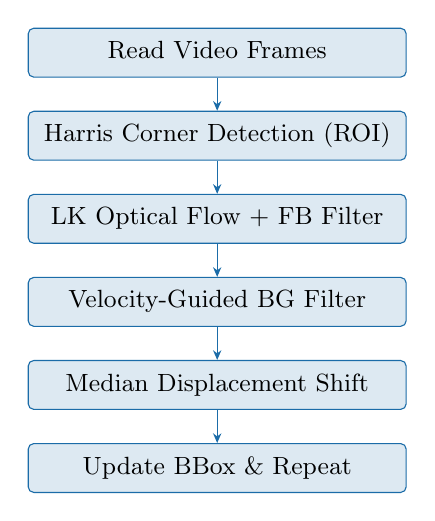
\begin{tikzpicture}[
  node distance=0.42cm,
  block/.style={rectangle, draw=accentteal, fill=accentteal!15, thin,
                minimum width=4.8cm, minimum height=0.60cm,
                font=\small\strut, align=center, rounded corners=2pt},
  arrow/.style={-{Stealth[length=3.5pt,width=3pt]}, thin, color=accentteal},
]
  \node[block] (A) {Read Video Frames};
  \node[block, below=of A] (B) {Harris Corner Detection (ROI)};
  \node[block, below=of B] (C) {LK Optical Flow + FB Filter};
  \node[block, below=of C] (D) {Velocity-Guided BG Filter};
  \node[block, below=of D] (E) {Median Displacement Shift};
  \node[block, below=of E] (F) {Update BBox \& Repeat};
  \draw[arrow] (A)--(B);
  \draw[arrow] (B)--(C);
  \draw[arrow] (C)--(D);
  \draw[arrow] (D)--(E);
  \draw[arrow] (E)--(F);
\end{tikzpicture}
\end{center}

\vspace{1.5cm}

{\centering
\begin{tabular}{rl}
  \textbf{Submitted by:} & Ali Ahmad \quad (Roll No.\ 23L-2619)\\[4pt]
  \textbf{Instructor:}   & Mubasher Baig\\[4pt]
  \textbf{Date:}         & May 2026\\
\end{tabular}
\par}

\vfill
\noindent\textcolor{accentteal}{\rule{\linewidth}{1pt}}

\end{titlepage}

% --- Abstract (roman numeral ii, own page) ------------------
\clearpage
\pagenumbering{roman}
\setcounter{page}{2}
\thispagestyle{plain}

\noindent{\large\bfseries\color{reportblue} Abstract}\\[-4pt]
\noindent\textcolor{accentteal}{\rule{\textwidth}{1.2pt}}
\vspace{4pt}

\begin{mdframed}[
  linecolor=accentteal,
  linewidth=0.8pt,
  roundcorner=5pt,
  innertopmargin=12pt,
  innerbottommargin=12pt,
  innerleftmargin=14pt,
  innerrightmargin=14pt,
  backgroundcolor=accentteal!6,
  skipabove=0pt,
  skipbelow=0pt,
]
\noindent
Object tracking in high-resolution video remains a fundamental challenge in computer vision,
particularly when deep-learning pipelines are unavailable or computationally prohibitive.
This report presents a classical feature-based single-object tracker that combines Harris
corner detection with pyramidal Lucas--Kanade (LK) optical flow to track diverse objects in
high-resolution footage, entirely without a Kalman filter or any learned component.

The system operates in six stages: Harris corners are initialised inside a user-defined bounding
box on the first frame; the pyramidal LK tracker propagates those points forward; a forward--
backward error check discards unreliable correspondences; a per-frame motion filter removes
stationary background corners; the bounding box is updated via median displacement shift; and,
when corner survival falls below a configurable threshold, the tracker redetects anchors on the
visible object region. Additional robustness comes from CLAHE preprocessing and a velocity
prediction mechanism that carries the bounding box forward when corner count drops critically
low.

The system was evaluated on six test sequences spanning diverse object types and camera
conditions: two 4K vehicle sequences (drone and surveillance), a static-camera rolling ball clip,
a handheld panning ball clip, a handheld walking-person clip, and a handheld flying eagle clip.
Tests 1 and 2 (textured vehicles, static or controlled camera) achieved 100\% tracker stability
with average point counts of $\approx$41 and 137, respectively. Tests 3--6 deliberately pushed the
system beyond its design boundary, exposing the fundamental limitations of the Harris corner
model when applied to smooth textureless objects and handheld footage with ego-motion.
Results demonstrate robust performance on structured scenarios and provide academically
rigorous documentation of failure modes for smooth, fast-moving, and ego-motion-corrupted
scenes.

\medskip
\textbf{Keywords:} Harris corner detector, Lucas--Kanade optical flow, forward--backward error,
CLAHE, single-object tracking, 4K video, textureless objects, ego-motion.
\end{mdframed}

% --- Table of Contents (own page, roman numerals) -----------
\clearpage
\thispagestyle{plain}
\tableofcontents

\clearpage
\pagenumbering{arabic}
\setcounter{page}{1}

% ============================================================
\section{Introduction}
% ============================================================
Object tracking is the task of continuously estimating the position (and optionally the extent)
of a target entity across sequential video frames. It underpins a wide range of real-world
applications: intelligent surveillance systems use it to maintain person or vehicle identity across
camera views; autonomous vehicle perception stacks rely on it to associate sensor detections
over time; unmanned aerial vehicles use it to follow a ground target or avoid dynamic obstacles;
and sports analytics platforms use it to compute player statistics from broadcast footage. In all
these domains, tracking must operate reliably under scale changes, illumination shifts, partial
occlusion, motion blur, and background clutter.

\subsection{Problem Statement}
This project addresses single-object tracking of diverse targets in high-resolution video using
only classical computer vision methods. The assignment specification explicitly prohibits
deep-learning-based detectors, Kalman-filter state estimation, or any form of learned feature
representation. The chosen approach --- Harris corner detection followed by pyramidal Lucas--
Kanade optical flow --- is lightweight and interpretable, but introduces several non-trivial
challenges:
\begin{itemize}[leftmargin=1.5em]
  \item \textbf{Uniform object texture.} The silver car roof (test~1) and smooth ball surfaces
    (tests~3, 4) provide very few high-response Harris corners.
  \item \textbf{Stationary background competition.} Road markings, tarmac cracks, and
    wall/car edges produce Harris responses that the LK tracker picks up and carries.
  \item \textbf{Camera ego-motion.} Handheld footage (tests~4, 5, 6) introduces global
    optical flow that corrupts the median displacement estimate.
  \item \textbf{Fast inter-frame displacement.} At 30\,fps with fast-moving objects, the
    LK search pyramid may be insufficient to bridge the gap between frames.
  \item \textbf{Point degradation at frame exit.} As the object approaches the frame boundary
    (test~2), corners progressively leave the image.
\end{itemize}

\subsection{Motivation}
Deep-learning trackers such as SiamRPN~\cite{siamrpn} or transformer-based architectures
achieve state-of-the-art accuracy on benchmark datasets, but they demand GPUs, large training
corpora, and opaque inference pipelines. Classical feature-based tracking, by contrast, is fully
interpretable --- every decision has a direct geometric meaning --- and can run on commodity
hardware. Studying these foundations rigorously is therefore both pedagogically and practically
valuable, particularly in understanding \emph{when} and \emph{why} such methods fail.

\subsection{Proposed System}
To address the challenges above, the system introduces three key extensions on top of the
standard Harris + LK pipeline:
\begin{enumerate}[leftmargin=1.8em]
  \item \textbf{Per-frame motion-based background filter.} Each frame, per-point
    displacement magnitudes are computed directly from the LK point cloud; any point
    moving less than \texttt{min\_motion\_threshold} px/frame is discarded as likely
    static background.
  \item \textbf{Survival-based redetection.} Rather than redetecting on a fixed schedule,
    the tracker monitors the ratio of surviving points to initial count; redetection triggers
    whenever this ratio drops below a configurable threshold.
  \item \textbf{Velocity prediction.} When surviving points fall below the minimum required
    threshold, the tracker blends measured displacement with an exponentially smoothed
    velocity estimate to keep the bounding box moving forward.
\end{enumerate}
CLAHE~\cite{clahe} preprocessing is applied at both the Harris detection and LK tracking
stages to normalise local contrast and improve corner repeatability under varying illumination.

\subsection{Scope}
The system is evaluated on six test videos: two 4K vehicle sequences (test~1: drone,
280~frames at 24\,fps; test~2: surveillance, 529~frames at 30\,fps) representing the
successful-tracking regime, and four portrait-orientation sequences at 30\,fps (test~3:
static rolling ball, 156~frames; test~4: handheld panning ball, 190~frames; test~5:
handheld walking person, 504~frames; test~6: handheld flying eagle, 567~frames) that
systematically expose the algorithmic limits of texture-based classical tracking.

% ============================================================
\section{Related Work}
% ============================================================

\textbf{Classical correlation and feature-based trackers.}
The MOSSE filter~\cite{mosse} demonstrated that correlation filters operating in the frequency
domain could track at over 600\,fps on standard hardware. Kernelised Correlation Filters
(KCF)~\cite{kcf} extended this to multi-channel HOG features, achieving state-of-the-art
accuracy on the VOT2013 benchmark while remaining GPU-free. OpenCV's CSRT
tracker~\cite{csrt} refined KCF with a discriminative correlation filter that handles
shape-irregular objects and partial occlusion. The present work deliberately avoids these
correlation-filter approaches to maintain full geometric interpretability.

\textbf{Optical flow and point-based tracking.}
Shi and Tomasi~\cite{shitomasi} showed that selecting corners by the minimum eigenvalue
of the second-moment matrix improved tracking stability; their \texttt{goodFeaturesToTrack}
API underpins the detection stage of this project. Farneb\"{a}ck's dense optical
flow~\cite{farneback} computes a per-pixel polynomial-expansion flow field, offering richer
displacement information than sparse LK but at a cost of $\mathcal{O}(HW)$ complexity per
frame, prohibitive for 4K footage without GPU acceleration.

\textbf{Deep learning trackers.}
SiamRPN~\cite{siamrpn} reformulated tracking as a cross-correlation localisation task on
Siamese backbone features. Subsequent transformer-based architectures achieve near-perfect
scores on the LaSOT~\cite{lasot} and GOT-10k benchmarks. While these methods set the
accuracy bar, they require pre-trained weights on millions of bounding-box annotations and
cannot run at acceptable speed without a dedicated GPU.

\textbf{UAV and surveillance tracking.}
Mueller et al.~\cite{uavbenchmark} introduced a dedicated UAV tracking benchmark showing
that top-down aerial footage poses unique challenges: perspective foreshortening causes objects
to appear as textureless blobs, and rapid ego-motion introduces global optical flow that naive
trackers confuse with object motion. Marvasti-Zadeh et al.~\cite{marvasti} survey deep
trackers on aerial datasets, confirming that classical methods remain competitive on structured
scenarios where motion is predictable and background clutter is limited.

\textbf{Limitations of texture-based tracking.}
The failure of Harris-based methods on smooth textureless objects is mathematically
well-understood. The Harris corner response $R = \det(M) - k\,(\mathrm{tr}\,M)^2$ requires
non-zero gradient magnitude in two orthogonal directions; a smooth sphere or a uniformly
coloured cloth surface produces $M \approx \mathbf{0}$ everywhere in the interior, yielding
$R \approx 0$. Alternative approaches such as Hough circle detection~\cite{hough},
colour-based segmentation, or learned appearance models (e.g.\ ByteTrack~\cite{bytetrack})
are required for such objects.

% ============================================================
\section{Methodology}
% ============================================================

\subsection{Harris Corner Detection}
Harris and Stephens~\cite{harris} define corner strength via the second-moment matrix $M$
of image gradients:
\[
  M = \sum_{(x,y)\in\mathcal{W}} w(x,y)
  \begin{pmatrix} I_x^2 & I_xI_y \\ I_xI_y & I_y^2 \end{pmatrix},
\]
where $I_x,I_y$ are spatial derivatives and $w$ is a Gaussian weighting window. The corner
response is $R = \det(M) - k\,(\mathrm{tr}\,M)^2$, $k=0.04$. Points with $R$ above a
quality-scaled threshold are accepted. In this system, \texttt{cv2.goodFeaturesToTrack}
is used with \texttt{useHarrisDetector=True}. Detection is masked to the user-defined
bounding box using an eroded binary mask. CLAHE enhancement is applied before detection.

\subsection{Lucas--Kanade Pyramidal Optical Flow}
The Lucas--Kanade method~\cite{lucas} assumes brightness constancy and spatial coherence
within a local window $\mathcal{W}$ to solve for the flow vector $\mathbf{v}=(v_x,v_y)^\top$:
\[
  \mathbf{v} = \left(\sum_{\mathcal{W}} \nabla I\, \nabla I^\top\right)^{-1}
               \left(-\sum_{\mathcal{W}} I_t\, \nabla I\right).
\]
Bouguet's pyramidal extension~\cite{bouguet} resolves large inter-frame displacements by
computing flow coarse-to-fine across an image pyramid. The forward--backward error check
accepts point $p_t$ only if $\|p_t - \tilde{p}_t\| < \epsilon_{\text{fb}}$ where $\tilde{p}_t$
is the back-tracked prediction from $\hat{p}_{t+1}$.

\subsection{Motion-Based Background Filtering}

Two complementary motion filtering strategies are employed across the six test sequences,
targeting the same goal --- suppression of static background corners from the displacement vote
--- but differing in their reference signal.

\textbf{Method~1: EMA velocity filter (Tests~1 and~2).}
When tracking well-textured objects under controlled camera conditions, the tracker maintains
a reliable exponential moving average (EMA) velocity estimate
$\mathbf{v}^e_t = \alpha\,\Delta\mathbf{b}_t + (1-\alpha)\,\mathbf{v}^e_{t-1}$
($\alpha = 0.6$), where $\Delta\mathbf{b}_t$ is the frame-to-frame bbox displacement.
A point $p_i$ is retained if its displacement magnitude $\delta_i$ exceeds approximately
30\,\% of the estimated object speed $\|\mathbf{v}^e_t\|$.
This adaptive threshold scales automatically with object velocity and is reliable when the
bbox velocity estimate is trustworthy --- i.e.\ when the tracker is locked on the object.
For Tests~1 and~2 (vehicle sequences with 41--137 on-object corners), this condition holds
throughout the sequence.

\textbf{Method~2: Per-frame displacement magnitude filter (Tests~3--6).}
When the bbox velocity estimate cannot be trusted --- because the tracker has drifted onto
background features, because ego-motion corrupts the displacement history, or because point
counts are too low to form a stable EMA --- the system switches to a frame-local filter.
Let $\delta_i = \|\hat{p}^i_{t+1} - p^i_t\|$ denote the raw LK displacement of the
$i$-th point in the current frame. Points with $\delta_i < \theta_{\text{motion}}$
(configurable \texttt{min\_motion\_threshold}, set to 0.8--5.0\,px/frame depending on the
test) are classified as stationary background and excluded from the median displacement vote.
This approach bypasses bbox history entirely, making it robust to corrupted velocity estimates.
It was introduced specifically to address test~4, where the EMA velocity decayed to zero
after the bbox froze on background features, causing the EMA filter to stop firing even while
the ball was still moving at 15--20\,px/frame.

\subsection{Bounding-Box Update}
The bounding-box origin is shifted by the median displacement of surviving, filtered points:
$(x_{t+1}, y_{t+1}) = (x_t + \tilde{\Delta x},\; y_t + \tilde{\Delta y})$,
where $\tilde{\Delta x}, \tilde{\Delta y}$ are component-wise medians.

\subsection{Survival-Based Redetection}
Let $N_0$ be the point count at initialisation and $N_t$ the count at frame $t$. If
$N_t/N_0 < \rho$ (configurable \texttt{redetect\_threshold}), new Harris corners are detected
inside the current bounding box and $N_0$ is reset to $N_t$.

\subsection{Velocity Prediction}
When $N_t < N_{\min}$, the tracker enters prediction mode. If at least one point survives,
measured and velocity-predicted displacements are blended with weight
$w = \max(0, N_t/N_{\min}-1)$. If zero points survive, the bounding box is advanced by the raw
EMA velocity estimate $\mathbf{v}^e$ (smoothed with $\alpha=0.6$).

% ============================================================
\section{System Architecture}
% ============================================================

\subsection{Codebase Structure}
The project is organised as a modular Python package under \texttt{cv\_project/}.
Figure~\ref{fig:projstruct} shows the full directory and module layout; each layer is
described in Table~\ref{tab:modules}.

\begin{figure}[H]
\centering
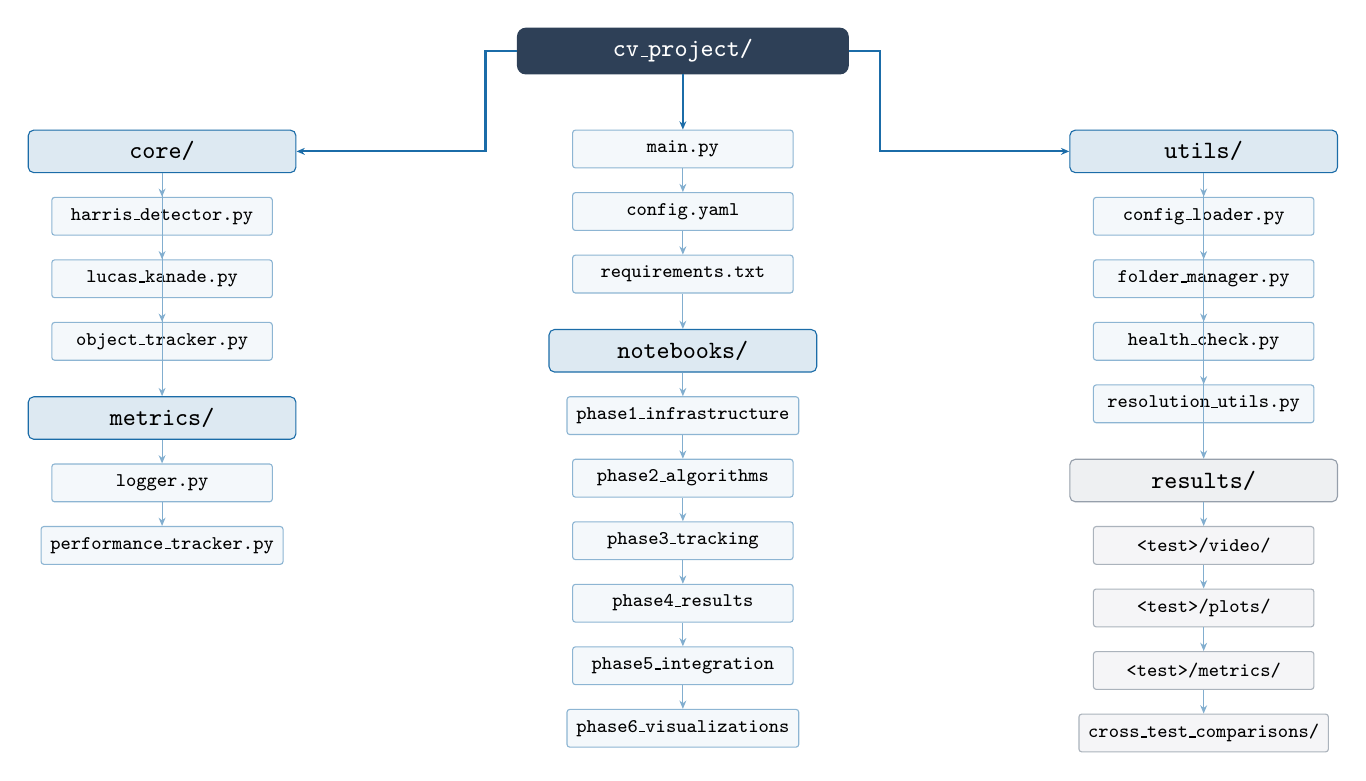
\begin{tikzpicture}[
  node distance=0.30cm and 0.5cm,
  root/.style={rectangle, draw=reportblue, fill=reportblue, text=white,
               font=\small\bfseries, rounded corners=3pt,
               minimum width=4.2cm, minimum height=0.58cm, align=center},
  pkg/.style={rectangle, draw=accentteal, fill=accentteal!15,
              font=\small\bfseries, rounded corners=2pt,
              minimum width=3.4cm, minimum height=0.54cm, align=center},
  file/.style={rectangle, draw=accentteal!50, fill=accentteal!5,
               font=\scriptsize\ttfamily, rounded corners=1pt,
               minimum width=2.8cm, minimum height=0.48cm, align=center},
  outpkg/.style={rectangle, draw=reportblue!50, fill=reportblue!8,
                 font=\small\bfseries, rounded corners=2pt,
                 minimum width=3.4cm, minimum height=0.54cm, align=center},
  outfile/.style={rectangle, draw=reportblue!40, fill=reportblue!5,
                  font=\scriptsize\ttfamily, rounded corners=1pt,
                  minimum width=2.8cm, minimum height=0.48cm, align=center},
  arr/.style={-{Stealth[length=3pt,width=2.5pt]}, thick, color=accentteal},
  darr/.style={-{Stealth[length=3pt,width=2.5pt]}, thin, color=accentteal!55},
]

%% ROOT
\node[root] (root) {\texttt{cv\_project/}};

%% --- LEFT COLUMN: Core packages ---
\node[pkg, below left=0.7cm and 2.8cm of root]  (core)   {\texttt{core/}};
\node[file, below=of core]  (hd)  {harris\_detector.py};
\node[file, below=of hd]    (lk)  {lucas\_kanade.py};
\node[file, below=of lk]    (ot)  {object\_tracker.py};

\node[pkg, below=0.45cm of ot]   (metrics) {\texttt{metrics/}};
\node[file, below=of metrics]    (log)  {logger.py};
\node[file, below=of log]        (pt)   {performance\_tracker.py};

%% --- CENTRE COLUMN: Config + entry point ---
\node[file, below=0.7cm of root, xshift=0.0cm]   (main)   {main.py};
\node[file, below=of main]                         (cfg)    {config.yaml};
\node[file, below=of cfg]                          (req)    {requirements.txt};

\node[pkg, below=0.45cm of req]   (nb) {\texttt{notebooks/}};
\node[file, below=of nb]   (nb1) {phase1\_infrastructure};
\node[file, below=of nb1]  (nb2) {phase2\_algorithms};
\node[file, below=of nb2]  (nb3) {phase3\_tracking};
\node[file, below=of nb3]  (nb4) {phase4\_results};
\node[file, below=of nb4]  (nb5) {phase5\_integration};
\node[file, below=of nb5]  (nb6) {phase6\_visualizations};

%% --- RIGHT COLUMN: Utils + results ---
\node[pkg, below right=0.7cm and 2.8cm of root]  (utils)  {\texttt{utils/}};
\node[file, below=of utils] (cl) {config\_loader.py};
\node[file, below=of cl]    (fm) {folder\_manager.py};
\node[file, below=of fm]    (hc) {health\_check.py};
\node[file, below=of hc]    (ru) {resolution\_utils.py};

\node[outpkg, below=0.45cm of ru] (res) {\texttt{results/}};
\node[outfile, below=of res]  (rv)  {<test>/video/};
\node[outfile, below=of rv]   (rp)  {<test>/plots/};
\node[outfile, below=of rp]   (rm)  {<test>/metrics/};
\node[outfile, below=of rm]   (rc)  {cross\_test\_comparisons/};

%% Arrows from root to top-level nodes
\draw[arr] (root.west)  -- ++(-0.4,0) |- (core.east);
\draw[arr] (root.south) -- (main.north);
\draw[arr] (root.east)  -- ++(0.4,0)  |- (utils.west);

%% Core children
\draw[darr] (core.south) -- (hd.north);
\draw[darr] (hd.south)   -- (lk.north);
\draw[darr] (lk.south)   -- (ot.north);
\draw[darr] (core.south) -- ++(0,-0.1) -| (metrics.north);

%% Metrics children
\draw[darr] (metrics.south) -- (log.north);
\draw[darr] (log.south)     -- (pt.north);

%% Centre children
\draw[darr] (main.south) -- (cfg.north);
\draw[darr] (cfg.south)  -- (req.north);
\draw[darr] (req.south)  -- ++(0,-0.1) -- (nb.north);
\draw[darr] (nb.south) -- (nb1.north);
\draw[darr] (nb1.south) -- (nb2.north);
\draw[darr] (nb2.south) -- (nb3.north);
\draw[darr] (nb3.south) -- (nb4.north);
\draw[darr] (nb4.south) -- (nb5.north);
\draw[darr] (nb5.south) -- (nb6.north);

%% Utils children
\draw[darr] (utils.south) -- (cl.north);
\draw[darr] (cl.south)    -- (fm.north);
\draw[darr] (fm.south)    -- (hc.north);
\draw[darr] (hc.south)    -- (ru.north);
\draw[darr] (utils.south) -- ++(0,-0.1) -| (res.north);

%% Results children
\draw[darr] (res.south) -- (rv.north);
\draw[darr] (rv.south)  -- (rp.north);
\draw[darr] (rp.south)  -- (rm.north);
\draw[darr] (rm.south)  -- (rc.north);

\end{tikzpicture}
\caption{Project directory and module structure. Blue root node is the package root;
teal nodes are sub-packages; white nodes are individual files. The \texttt{results/}
subtree (blue-tinted) is generated at runtime and not part of the source tree.}
\label{fig:projstruct}
\end{figure}

\begin{table}[H]
\centering
\caption{Module responsibilities in the \texttt{cv\_project} package.}
\label{tab:modules}
\small
\renewcommand{\arraystretch}{1.12}
\begin{tabularx}{\textwidth}{lX}
\toprule
\rowcolor{accentteal!20}
\textbf{Module} & \textbf{Responsibility} \\
\midrule
\texttt{core/harris\_detector.py} & Harris corner detector with CLAHE preprocessing \& eroded bbox mask \\
\texttt{core/lucas\_kanade.py} & Pyramidal LK tracker with forward--backward error filtering \\
\texttt{core/object\_tracker.py} & Stateful single-object tracker: motion filter, redetection, velocity prediction \\
\texttt{metrics/logger.py} & Levelled logging (INFO / DEBUG / WARNING) with timestamped output \\
\texttt{metrics/performance\_tracker.py} & Per-frame metric accumulation, JSON export, and summary generation \\
\texttt{utils/config\_loader.py} & YAML configuration loader with dot-access attribute syntax \\
\texttt{utils/folder\_manager.py} & Timestamped per-run output directory creation and management \\
\texttt{utils/health\_check.py} & Pre-flight environment validation (OpenCV version, paths, dependencies) \\
\texttt{utils/resolution\_utils.py} & Frame resolution helper utilities for downscaling and aspect ratio \\
\texttt{main.py} & CLI entry point; wires config, video source, tracker, and output writer \\
\texttt{config.yaml} & All tunable parameters; only \texttt{source}, \texttt{start\_frame}, \texttt{bbox} change per test \\
\texttt{notebooks/phase1--6} & Phased development notebooks: infrastructure through full integration \\
\texttt{results/<test>/} & Runtime output: tracked video, per-frame metrics JSON, diagnostic plots \\
\bottomrule
\end{tabularx}
\end{table}

\subsection{System Pipeline Diagram}

Figure~\ref{fig:pipeline} shows the complete per-frame tracking loop as implemented in
\texttt{object\_tracker.py}, called from \texttt{main.py}. Harris corner detection fires
only at initialisation and on survival-triggered redetection --- \emph{not} on every frame.
The per-frame loop drives purely on LK optical flow from the previously established anchor set.

\begin{figure}[H]
\centering
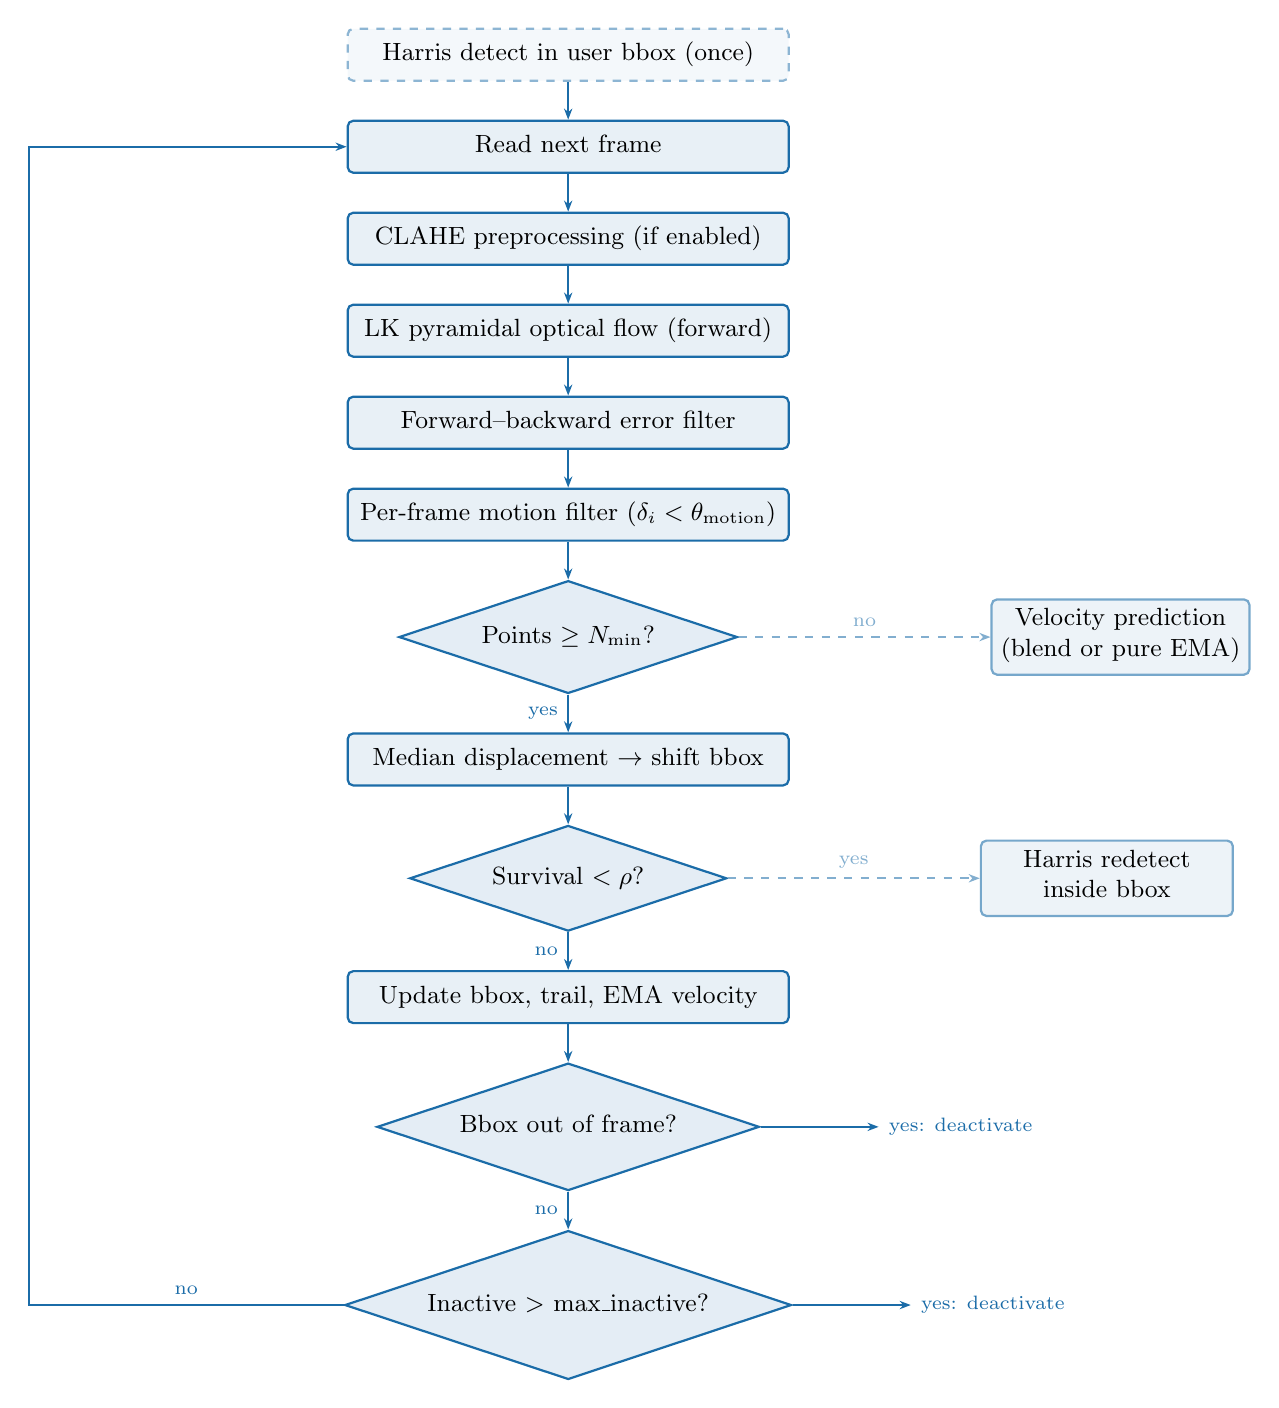
\begin{tikzpicture}[
  node distance=0.48cm and 2.6cm,
  block/.style={rectangle, draw=accentteal, fill=accentteal!10, thick,
                minimum width=5.6cm, minimum height=0.66cm,
                font=\small\strut, align=center, rounded corners=2pt},
  initblock/.style={rectangle, draw=accentteal!50, fill=accentteal!5, thick,
                minimum width=5.6cm, minimum height=0.66cm,
                font=\small\strut, align=center, rounded corners=2pt, dashed},
  decision/.style={diamond, draw=accentteal, fill=accentteal!12, thick,
                   aspect=3.0, font=\small\strut, align=center},
  sideblock/.style={rectangle, draw=accentteal!60, fill=accentteal!8, thick,
                minimum width=3.2cm, minimum height=0.66cm,
                font=\small\strut, align=center, rounded corners=2pt},
  arrow/.style={-{Stealth[length=4pt,width=3pt]}, thick, color=accentteal},
  darrow/.style={-{Stealth[length=4pt,width=3pt]}, thick, color=accentteal!55, dashed},
]
  % One-time initialisation
  \node[initblock]             (I)  {Harris detect in user bbox (once)};
  % Per-frame loop
  \node[block, below=of I]     (A)  {Read next frame};
  \node[block, below=of A]     (B)  {CLAHE preprocessing (if enabled)};
  \node[block, below=of B]     (C)  {LK pyramidal optical flow (forward)};
  \node[block, below=of C]     (D)  {Forward--backward error filter};
  \node[block, below=of D]     (E)  {Per-frame motion filter ($\delta_i < \theta_{\text{motion}}$)};
  \node[decision, below=of E]  (d1) {Points $\geq N_{\min}$?};
  \node[block, below=of d1]    (G)  {Median displacement $\rightarrow$ shift bbox};
  \node[decision, below=of G]  (d2) {Survival $< \rho$?};
  \node[block, below=of d2]    (H)  {Update bbox, trail, EMA velocity};
  \node[decision, below=of H]  (d3) {Bbox out of frame?};
  \node[decision, below=of d3] (d4) {Inactive $>$ max\_inactive?};

  % Side blocks
  \node[sideblock, right=of d1, xshift=0.6cm] (Pred)
        {Velocity prediction\\(blend or pure EMA)};
  \node[sideblock, right=of d2, xshift=0.6cm] (Redet)
        {Harris redetect\\inside bbox};

  % Flows
  \draw[arrow] (I)--(A);
  \draw[arrow] (A)--(B);
  \draw[arrow] (B)--(C);
  \draw[arrow] (C)--(D);
  \draw[arrow] (D)--(E);
  \draw[arrow] (E)--(d1);
  \draw[arrow] (d1)--node[left,font=\scriptsize]{yes}(G);
  \draw[arrow] (G)--(d2);
  \draw[arrow] (d2)--node[left,font=\scriptsize]{no}(H);
  \draw[arrow] (H)--(d3);
  \draw[arrow] (d3)--node[left,font=\scriptsize]{no}(d4);

  % Side branches
  \draw[darrow] (d1.east)--node[above,font=\scriptsize]{no}(Pred.west);
  \draw[darrow] (d2.east)--node[above,font=\scriptsize]{yes}(Redet.west);

  % Deactivate exits
  \draw[arrow] (d3.east) -- ++(1.5,0)
    node[right,font=\scriptsize,color=accentteal]{yes: deactivate};
  \draw[arrow] (d4.east) -- ++(1.5,0)
    node[right,font=\scriptsize,color=accentteal]{yes: deactivate};

  % Loop back (next frame)
  \draw[arrow] (d4.west) -- ++(-4.0,0)
    node[midway,above,font=\scriptsize]{no}
    |- (A.west);
\end{tikzpicture}
\caption{Per-frame tracking pipeline (\texttt{object\_tracker.py}). Dashed box: Harris detection
runs once at initialisation and again on survival-triggered redetection. Dashed arrows: side
branches for velocity prediction ($N < N_{\min}$) and Harris redetection (survival $< \rho$).
Two exit conditions deactivate the tracker: bbox leaving the frame boundary, or exceeding
\texttt{max\_inactive\_frames} consecutive low-point frames.}
\label{fig:pipeline}
\end{figure}

\subsection{Configuration-Driven Design}
All parameters are centralised in \texttt{config.yaml}. Only three fields change between test
videos: \texttt{source}, \texttt{start\_frame}, and \texttt{bbox}. This separation ensures
reproducibility and makes ablation studies straightforward.

% ============================================================
\section{Implementation Details}
% ============================================================

\subsection{Parameter Table}

Table~\ref{tab:params} lists all key parameters with their values for each test and rationale.

\begin{table}[H]
\centering
\caption{System parameters across all six test runs.}
\label{tab:params}
\scriptsize
\renewcommand{\arraystretch}{1.15}
\setlength{\tabcolsep}{4pt}
\begin{tabular}{l p{1.25cm} p{1.25cm} p{1.25cm} p{1.25cm} p{1.25cm} p{1.25cm}}
\toprule
\rowcolor{accentteal!20}
\textbf{Parameter} & \textbf{Test 1} & \textbf{Test 2} & \textbf{Test 3} & \textbf{Test 4} & \textbf{Test 5} & \textbf{Test 6} \\
\midrule
\multicolumn{7}{l}{\textit{Harris Corner Detection}} \\
\quad max\_corners & 400 & 400 & 500 & 50 & 300 & 20 \\
\quad quality\_level & 0.005 & 0.005 & 0.001 & 0.001 & 0.010 & 0.005 \\
\quad min\_distance & 3 & 3 & 2 & 2 & 8 & 3 \\
\quad block\_size & 5 & 5 & 3 & 3 & 5 & 3 \\
\quad k & 0.04 & 0.04 & 0.04 & 0.04 & 0.04 & 0.04 \\
\midrule
\multicolumn{7}{l}{\textit{Lucas--Kanade Optical Flow}} \\
\quad win\_size & $41\times41$ & $41\times41$ & $41\times41$ & $61\times61$ & $31\times31$ & $11\times11$ \\
\quad max\_level & 5 & 5 & 5 & 6 & 4 & 3 \\
\quad fb\_error\_thresh & 3.5 & 3.5 & 3.0 & 10.0 & 1.5 & 2.0 \\
\midrule
\multicolumn{7}{l}{\textit{Tracking Logic}} \\
\quad min\_points & 4 & 4 & 4 & 3 & 4 & 3 \\
\quad redetect\_thresh & 0.25 & 0.25 & 0.25 & 0.60 & 0.25 & 0.30 \\
\quad redetect\_interval & 60 & 60 & 60 & 60 & 10 & 60 \\
\quad min\_motion\_thr & 0.8 & 0.8 & 0.8 & 2.0 & 0.8 & 0.8 \\
\quad bbox\_smoothing & 0.0 & 0.0 & 0.0 & 0.0 & 0.0 & 0.0 \\
\midrule
\multicolumn{7}{l}{\textit{Preprocessing}} \\
\quad CLAHE enabled & Yes & Yes & Yes & Yes & No & Yes \\
\quad clip limit & 4.0 & 4.0 & 2.0 & 5.0 & --- & 4.0 \\
\quad tile size & $4\times4$ & $4\times4$ & $8\times8$ & $2\times2$ & --- & $4\times4$ \\
\midrule
\multicolumn{7}{l}{\textit{Video / Bbox}} \\
\quad start\_frame & 0 & 0 & 21 & 38 & 0 & 0 \\
\quad bbox $x$ & --- & --- & 707 & 381 & 548 & 529 \\
\quad bbox $y$ & --- & --- & 832 & 1520 & 469 & 462 \\
\quad bbox $w\times h$ & --- & --- & $59\times101$ & $160\times253$ & $110\times280$ & $11\times26$ \\
\bottomrule
\end{tabular}
\end{table}

\subsection{Key Design Decisions}

\textbf{Median over mean.} The median displacement is used because occasional outlier
correspondences that pass the FB filter would significantly bias the mean. The median is
inherently robust to such outliers without requiring an additional RANSAC step.

\textbf{Survival-based vs.\ scheduled redetection.} Early versions redetected on a fixed
interval (every 60 frames). This caused unnecessary restarts in stable phases and delayed
redetection in rapid-loss phases. The survival ratio trigger makes redetection purely
data-driven. For test~5, a very short redetect\_interval of 10 frames was trialled to cope
with clothing deformation, but still could not overcome background dominance.

\textbf{No bbox smoothing.} Setting \texttt{bbox\_smoothing\,=\,0} lets the bounding box
follow the object exactly each frame. Temporal averaging would reduce jitter but introduce
lag that becomes visible at high object speeds.

\textbf{Per-frame motion filter vs.\ EMA filter.} The original velocity-EMA background
filter checked whether per-point speed exceeded a fraction of the EMA bbox velocity. Once
the bbox froze (e.g.\ tracking background in test~3), the EMA velocity decayed to zero and
the filter stopped firing. The replacement per-frame filter computes displacement magnitudes
directly from each frame's LK result, bypassing bbox history entirely.

\subsection{Hyperparameter Sensitivity Analysis}

Tables~\ref{tab:hyper2}--\ref{tab:hyper6} document every parameter trial conducted across all six
tests. Figures~\ref{fig:hyper2} and~\ref{fig:hyper1} visualise the outcome differences for tests~1
and~2; Figure~\ref{fig:hyperss} shows the combined tuning chart. Tests~3 and~5 each used a single
configuration run (the root failure is mathematical, not parametric); tests~4 and~6 underwent
multiple iterative runs as documented in their respective tables.

\begin{table}[H]
\centering\small
\caption{Test~2 hyperparameter tuning history.}
\label{tab:hyper2}
\begin{tabularx}{\textwidth}{llX}
\toprule
\rowcolor{accentteal!20}
\textbf{Parameter} & \textbf{Value Tried} & \textbf{Observed Effect} \\
\midrule
\multirow{2}{*}{fb\_error\_threshold}
 & 2.0\,px & Too strict; rejected valid car-body points, count collapsed to 22 at frame 420 \\
 & 3.5\,px & Balanced; preserved valid car points throughout all 529 frames \\
\midrule
\multirow{2}{*}{redetect\_interval}
 & 30 frames & Fired too often; tracker locked onto background corners at frame 420 \\
 & 60 frames & Less frequent; rode on good corners longer without background drift \\
\midrule
\multirow{2}{*}{redetect\_threshold}
 & 0.40 & Triggered too early; caused premature background lock at high-survival frames \\
 & 0.25 & Stable; only triggered on genuine point loss \\
\midrule
\multirow{2}{*}{max\_inactive\_frames}
 & 20 & Only 0.67\,s tolerance at 30\,fps; tracker gave up before car fully exited \\
 & 45 & 1.5\,s grace window; followed object cleanly through the exit phase \\
\bottomrule
\end{tabularx}
\end{table}

\begin{table}[H]
\centering\small
\caption{Test~1 hyperparameter tuning history.}
\label{tab:hyper1}
\begin{tabularx}{\textwidth}{llX}
\toprule
\rowcolor{accentteal!20}
\textbf{Parameter} & \textbf{Value Tried} & \textbf{Observed Effect} \\
\midrule
\multirow{2}{*}{quality\_level}
 & 0.010 & Too few corners on the flat silver car roof ($<$10 in-bbox points) \\
 & 0.005 & More corners detected on uniform surface; 67 points at initialisation \\
\midrule
\multirow{2}{*}{bbox\_smoothing}
 & 0.25 & Bbox lagged behind fast-moving car; visible positional offset at 30\,fps \\
 & 0.0 & Bbox snapped directly to median shift each frame; zero lag \\
\midrule
\multirow{2}{*}{win\_size (width)}
 & $31\times31$ & Borderline for fast lateral motion; some valid flow vectors lost under blur \\
 & $41\times41$ & Handled up to 37\,px displacement per frame; minimum 36 points sustained \\
\bottomrule
\end{tabularx}
\end{table}

\begin{figure}[H]
\centering
\includegraphics[width=\textwidth]{imgs/cross/02_tracker_stability.png}
\caption{Test~2 hyperparameter tuning outcomes. Teal bars show the finally chosen value; red bars
show the suboptimal trial. The \texttt{fb\_error\_threshold} panel plots actual surviving point count;
the remaining panels use a binary success indicator (1\,=\,desirable outcome, 0\,=\,failure).}
\label{fig:hyper2}
\end{figure}

\begin{figure}[H]
\centering
\includegraphics[width=0.85\textwidth]{imgs/cross/03_harris_corners.png}
\caption{Test~1 hyperparameter tuning outcomes. \texttt{quality\_level} and \texttt{win\_size}
panels show corner/point counts; the \texttt{bbox\_smoothing} panel shows maximum observed lag in frames.}
\label{fig:hyper1}
\end{figure}

\begin{figure}[H]
\centering
\includegraphics[width=\textwidth]{hyper_screenshot.png}
\caption{Combined hyperparameter tuning outcome charts for Tests~1 and~2, as generated by the
project's visualisation pipeline. Each panel compares the suboptimal trial (red) against the
finally chosen value (teal).}
\label{fig:hyperss}
\end{figure}

\begin{table}[H]
\centering\small
\caption{Test~3 hyperparameter configuration (single run --- no successful tuning path exists within the Harris framework).}
\label{tab:hyper3}
\begin{tabularx}{\textwidth}{llX}
\toprule
\rowcolor{accentteal!20}
\textbf{Parameter} & \textbf{Value Used} & \textbf{Observed Effect} \\
\midrule
quality\_level & 0.001 & Most aggressive threshold available; still produced zero corners on ball surface; all 34 detected points came from wall and car edges \\
\midrule
max\_corners & 500 & Maximum set to 500; despite this, Harris found only 34 background corners; ball's smooth dark surface produces near-zero gradient response \\
\midrule
win\_size & $41\times41$ & Standard pyramid window; unable to bridge ball displacement of 46.55 mean px/frame (max 127) between frames 19--20 \\
\midrule
fb\_error\_threshold & 3.0\,px & Balanced setting; FB filter correctly rejected high-error correspondences, but all surviving 34 points were background features \\
\midrule
redetect\_interval & 60 frames & Each redetection re-anchored to the same 34 wall corners; no mechanism to redirect Harris toward the departed ball \\
\bottomrule
\end{tabularx}
\end{table}

\begin{table}[H]
\centering\small
\caption{Test~4 hyperparameter tuning history (six configuration runs).}
\label{tab:hyper4}
\begin{tabularx}{\textwidth}{llX}
\toprule
\rowcolor{accentteal!20}
\textbf{Parameter / Change} & \textbf{Value Tried} & \textbf{Observed Effect} \\
\midrule
\multirow{2}{*}{quality\_level}
 & 0.050 (Run~1) & Too strict for dark textureless ball; only 4--6 Harris points detected; tracker froze within 22 frames \\
 & 0.001 (Run~2+) & More permissive; point count rose to 500 at frame~60, stabilising at 130; all were concrete-crack corners \\
\midrule
\multirow{2}{*}{Adaptive bbox shrink}
 & Enabled (Runs~1--2) & Directional constraint \texttt{max(x, px1-pad)} blocked bbox from moving in the kick direction; tracker locked in place \\
 & Removed (Run~3+) & Bbox now free to move in all directions; but ego-motion issue then dominated \\
\midrule
\multirow{2}{*}{fb\_error\_threshold}
 & 3.5\,px (Run~1) & Too strict under motion blur; rejected valid correspondences \\
 & 10.0\,px (Run~6) & Relaxed to accommodate motion-blur-induced patch distortion at 30\,fps with fast kick \\
\midrule
\multirow{2}{*}{win\_size}
 & $41\times41$ (Run~1) & Insufficient for kick motion; valid flow vectors lost under blur \\
 & $61\times61$ (Run~6) & Larger search region; partially compensated fast inter-frame displacement \\
\midrule
\multirow{2}{*}{start\_frame}
 & 55 (Run~4, accidental) & 17-frame gap: ball had already left the bbox when tracking began; immediately detected wrong region \\
 & 38 (correct) & Bbox drawn at frame~38; correcting this removed the initialisation gap \\
\midrule
Motion filter & Accidentally removed (Run~4) & 500 ground corners passed straight into median calculation; zero net displacement produced a frozen bbox; re-inserting the four filter lines restored correct behaviour in Run~5 \\
\midrule
\multirow{2}{*}{Bbox size}
 & $265\times352$\,px (Runs~1--5) & Too large; flooded Harris with concrete cracks; background dominated median vote \\
 & $\approx130\times130$\,px (Run~6) & Tighter bbox reduced background contamination; final avg.\ 46.33 points/frame \\
\bottomrule
\end{tabularx}
\end{table}

\begin{table}[H]
\centering\small
\caption{Test~5 hyperparameter configuration (single reported run --- ego-motion is the root cause, not parameter values).}
\label{tab:hyper5}
\begin{tabularx}{\textwidth}{llX}
\toprule
\rowcolor{accentteal!20}
\textbf{Parameter} & \textbf{Value Used} & \textbf{Observed Effect} \\
\midrule
quality\_level & 0.010 & Moderate threshold; white clothing returns corners only at fabric edges and folds; 36 corners at initialisation, dropping to 15 by frame~120 \\
\midrule
fb\_error\_threshold & 1.5\,px & Tight setting to reject camera-shake-induced drift; also inadvertently rejected some valid clothing correspondences under handheld motion \\
\midrule
redetect\_interval & 10 frames & Aggressive redetection (every 0.33\,s) intended to re-acquire person after displacement; instead, each redetection re-anchored to background inside the drifted bbox, reinforcing background dominance \\
\midrule
win\_size & $31\times31$ & Smaller window chosen to limit flow reach under camera shake; resulted in fewer correspondences surviving the FB filter \\
\midrule
CLAHE & Disabled & Omitted for this test; white clothing has high inherent contrast, and CLAHE was found to saturate fabric highlights in preliminary inspection \\
\midrule
max\_corners & 300 & Set high to maximise clothing corner recovery; floor and wall corners dominated due to richer texture gradient \\
\bottomrule
\end{tabularx}
\end{table}

\begin{table}[H]
\centering\small
\caption{Test~6 hyperparameter tuning history (three configuration runs).}
\label{tab:hyper6}
\begin{tabularx}{\textwidth}{llX}
\toprule
\rowcolor{accentteal!20}
\textbf{Parameter / Change} & \textbf{Value Tried} & \textbf{Observed Effect} \\
\midrule
\multirow{2}{*}{quality\_level}
 & 0.010 (Run~1) & Too strict for eagle's $11\times26$\,px bbox after erosion; only 1--2 corners detected; tracker deactivated within 90 frames \\
 & 0.005 (Run~2+) & More permissive; tracker survived full 567 frames; corners on sky/cloud background near eagle's position \\
\midrule
\multirow{2}{*}{win\_size}
 & $41\times41$ (Run~1) & Over-reaching into sky background; wasted search area on a $11\times26$\,px object \\
 & $11\times11$ (Run~3) & Reduced to limit reach into surrounding sky; lower motion compensation range accepted as trade-off \\
\midrule
\multirow{2}{*}{max\_level}
 & 4 (Run~1) & Pyramid too deep for such a small bbox; coarser levels lost sub-pixel structure \\
 & 3 (Run~3) & Shallower pyramid matched the object scale; stabilised at 3 tracked points \\
\midrule
\multirow{2}{*}{fb\_error\_threshold}
 & 3.5\,px (Run~1) & Standard value; too strict given extreme displacement variance at 567 frames \\
 & 2.0\,px (Run~3) & Slightly tightened to reject wild sky correspondences while preserving the minimal 3-point set \\
\midrule
\multirow{2}{*}{min\_points}
 & 4 (Run~1) & Threshold too high for a $11\times26$\,px bbox; tracker immediately entered inactive counting \\
 & 3 (Run~2+) & Minimum viable set; allowed tracker to survive at the absolute floor of point count \\
\midrule
max\_inactive\_frames & 90 & Extended grace window essential; without it the tracker deactivated within the first 60-frame cycle of low-point events \\
\bottomrule
\end{tabularx}
\end{table}

% ============================================================
\section{Phase-by-Phase Analysis}
% ============================================================

The project was structured into six Jupyter notebook phases. Each phase isolated a specific
component of the pipeline, enabling independent validation before full integration.

% ------------------------------------------------------------
\subsection{Phase 1 --- Infrastructure}
% ------------------------------------------------------------

Phase~1 established the project skeleton: the YAML-based configuration loader (with
dot-accessible attributes via \texttt{config\_loader.py}), the timestamped output directory
manager (\texttt{folder\_manager.py}), and the levelled logger. The infrastructure was verified
by running a log-level test that emitted INFO, DEBUG, and WARNING messages and confirmed correct
timestamped file output in \texttt{results/}.

A key design decision was to centralise all parameters in \texttt{config.yaml} rather than
hardcoding values in individual modules. This means that switching from test~1 to any other test
requires editing only three lines in the config (source path, \texttt{start\_frame}, and
\texttt{bbox}), with zero code changes. The \texttt{health\_check.py} module performs pre-flight
environment validation to catch missing dependencies or incompatible OpenCV versions before any
processing begins.

% ------------------------------------------------------------
\subsection{Phase 2 --- Harris Corner Detection}
% ------------------------------------------------------------

Phase~2 implemented and validated the Harris corner detector on all six test videos. The detector
was configured via \texttt{config.yaml} and wrapped with CLAHE preprocessing and an eroded
bounding-box mask to restrict corner detection to the region of interest. Each test required
tuning of \texttt{quality\_level}, \texttt{max\_corners}, and \texttt{min\_distance} to balance
corner density against object-texture constraints.

\subsubsection*{\textit{Test 1 (Drone Footage --- Silver Car)}}

\begin{figure}[H]
\centering
\begin{subfigure}[b]{0.48\textwidth}
  
\includegraphics[width=\textwidth]{imgs/t1/p2/first_frame}
  \caption{First frame of test~1 with the user-defined bounding box overlaid on the silver car
  (3840$\times$2160, 24\,fps).}
\end{subfigure}\hfill
\begin{subfigure}[b]{0.48\textwidth}
  
\includegraphics[width=\textwidth]{imgs/t1/p2/harris_corners}
  \caption{Detected Harris corners (yellow dots) inside the bounding box on frame~0.
  66 corners initialised at \texttt{quality\_level}=0.005.}
\end{subfigure}
\caption{Phase~2: initial frame and corner initialisation for test~1.}
\label{fig:t1p2a}
\end{figure}

\begin{figure}[H]
\centering
\begin{subfigure}[b]{0.48\textwidth}
  
\includegraphics[width=\textwidth]{imgs/t1/p2/harris_response}
  \caption{Harris response map for test~1. Brighter\,=\,stronger corner response. The silver car
  roof shows weak response; strong corners concentrate on the car edges.}
\end{subfigure}\hfill
\begin{subfigure}[b]{0.48\textwidth}
  
\includegraphics[width=\textwidth]{imgs/t1/p2/quality_level_comparison}
  \caption{Effect of varying \texttt{quality\_level} on corner count. A low value of 0.005 is
  necessary to detect the sparse silver-roof corners; 0.01 drops the count below the reliable
  tracking threshold.}
\end{subfigure}
\caption{Phase~2: Harris response map and quality-level sensitivity for test~1.}
\label{fig:t1p2b}
\end{figure}

\subsubsection*{\textit{Test 2 (Surveillance Footage --- Oblique Car)}}

\begin{figure}[H]
\centering
\begin{subfigure}[b]{0.48\textwidth}
  
\includegraphics[width=\textwidth]{imgs/t2/p2/first_frame}
  \caption{First frame of test~2. The oblique surveillance angle exposes the car's side panels,
  windows, and wheel arches --- a much richer texture than the top-down drone view.}
\end{subfigure}\hfill
\begin{subfigure}[b]{0.48\textwidth}
  
\includegraphics[width=\textwidth]{imgs/t2/p2/harris_corners}
  \caption{Harris corners at initialisation for test~2. 201 corners detected at
  \texttt{quality\_level}=0.01, all concentrated on the car body.}
\end{subfigure}
\caption{Phase~2: initial frame and corner initialisation for test~2.}
\label{fig:t2p2a}
\end{figure}

\begin{figure}[H]
\centering
\begin{subfigure}[b]{0.48\textwidth}
  
\includegraphics[width=\textwidth]{imgs/t2/p2/harris_response}
  \caption{Harris response map for test~2. High-gradient edges on the car body, windows, and
  wheel arches produce strong, well-distributed corner responses.}
\end{subfigure}\hfill
\begin{subfigure}[b]{0.48\textwidth}
  
\includegraphics[width=\textwidth]{imgs/t2/p2/quality_level_comparison}
  \caption{Quality-level sensitivity for test~2. Unlike test~1, even higher thresholds retain
  ample corners due to the richer oblique-view surface texture.}
\end{subfigure}
\caption{Phase~2: Harris response map and quality-level sensitivity for test~2.}
\label{fig:t2p2b}
\end{figure}

\subsubsection*{\textit{Test 3 (Rolling Ball --- Static Camera)}}

\begin{figure}[H]
\centering
\begin{subfigure}[b]{0.48\textwidth}
  
\includegraphics[width=\textwidth]{imgs/t3/p2/first_frame}
  \caption{First frame of test~3. The bounding box (59$\times$101\,px at 1080$\times$1920
  portrait resolution) targets a small dark rolling ball in a courtyard.}
\end{subfigure}\hfill
\begin{subfigure}[b]{0.48\textwidth}
  
\includegraphics[width=\textwidth]{imgs/t3/p2/harris_corners}
  \caption{Harris corners for test~3. Despite \texttt{quality\_level}=0.001, all detected points
  originate from the background wall and car edges, not the ball surface.}
\end{subfigure}
\caption{Phase~2: initial frame and corner initialisation for test~3.}
\label{fig:t3p2a}
\end{figure}

\begin{figure}[H]
\centering
\begin{subfigure}[b]{0.48\textwidth}
  
\includegraphics[width=\textwidth]{imgs/t3/p2/harris_response}
  \caption{Harris response map for test~3. The ball region (dark smooth sphere) shows near-zero
  response while background structure shows strong responses --- the fundamental failure mode.}
\end{subfigure}\hfill
\begin{subfigure}[b]{0.48\textwidth}
  
\includegraphics[width=\textwidth]{imgs/t3/p2/quality_level_comparison}
  \caption{Quality-level sensitivity for test~3. No threshold produces corners on the ball
  surface; all detections are on the surrounding background regardless of parameter choice.}
\end{subfigure}
\caption{Phase~2: Harris response map and quality-level sensitivity for test~3.}
\label{fig:t3p2b}
\end{figure}

\subsubsection*{\textit{Test 4 (Handheld Panning --- Navy Blue Ball)}}

\begin{figure}[H]
\centering
\begin{subfigure}[b]{0.48\textwidth}
  
\includegraphics[width=\textwidth]{imgs/t4/p2/first_frame}
  \caption{First frame of test~4 at frame~38. The navy blue football (approx.\ 80--100\,px
  diameter) is tracked against a concrete surface with a panning handheld camera.}
\end{subfigure}\hfill
\begin{subfigure}[b]{0.48\textwidth}
  
\includegraphics[width=\textwidth]{imgs/t4/p2/harris_corners}
  \caption{Harris corners for test~4. 50 corners initialised at \texttt{quality\_level}=0.001;
  visual inspection confirms all originate from concrete cracks, not the ball surface.}
\end{subfigure}
\caption{Phase~2: initial frame and corner initialisation for test~4.}
\label{fig:t4p2a}
\end{figure}

\begin{figure}[H]
\centering
\begin{subfigure}[b]{0.48\textwidth}
  
\includegraphics[width=\textwidth]{imgs/t4/p2/harris_response}
  \caption{Harris response map for test~4. The concrete surface (cracks, joints, edges) dominates
  the response. The ball body produces near-zero Harris response due to its smooth, uniform
  navy surface.}
\end{subfigure}\hfill
\begin{subfigure}[b]{0.48\textwidth}
  
\includegraphics[width=\textwidth]{imgs/t4/p2/quality_level_comparison}
  \caption{Quality-level sensitivity for test~4. At every threshold, concrete-crack corners are
  preferentially detected over any ball-surface features.}
\end{subfigure}
\caption{Phase~2: Harris response map and quality-level sensitivity for test~4.}
\label{fig:t4p2b}
\end{figure}

\subsubsection*{\textit{Test 5 (Handheld Street --- Person in White Shalwar Kameez)}}

\begin{figure}[H]
\centering
\begin{subfigure}[b]{0.48\textwidth}
  
\includegraphics[width=\textwidth]{imgs/t5/p2/first_frame}
  \caption{First frame of test~5. The 110$\times$280\,px bounding box at frame~0 targets a person
  in white shalwar kameez on a handheld street-level video (1080$\times$1920, 30\,fps, 504 frames).}
\end{subfigure}\hfill
\begin{subfigure}[b]{0.48\textwidth}
  
\includegraphics[width=\textwidth]{imgs/t5/p2/harris_corners}
  \caption{Harris corners for test~5. 36 corners at initialisation, concentrated on clothing edges
  and fabric folds. White fabric has low internal texture; interior corners are near-absent.}
\end{subfigure}
\caption{Phase~2: initial frame and corner initialisation for test~5.}
\label{fig:t5p2a}
\end{figure}

\begin{figure}[H]
\centering
\begin{subfigure}[b]{0.48\textwidth}
  
\includegraphics[width=\textwidth]{imgs/t5/p2/harris_response}
  \caption{Harris response map for test~5. The white clothing shows only boundary-level responses;
  interior fabric texture is insufficient for reliable corner detection across frames.}
\end{subfigure}\hfill
\begin{subfigure}[b]{0.48\textwidth}
  
\includegraphics[width=\textwidth]{imgs/t5/p2/quality_level_comparison}
  \caption{Quality-level sensitivity for test~5. Higher thresholds rapidly deplete the already
  sparse corner set on the clothing, leaving insufficient points for stable tracking.}
\end{subfigure}
\caption{Phase~2: Harris response map and quality-level sensitivity for test~5.}
\label{fig:t5p2b}
\end{figure}

\subsubsection*{\textit{Test 6 (Handheld --- Flying Eagle)}}

\begin{figure}[H]
\centering
\begin{subfigure}[b]{0.48\textwidth}
  
\includegraphics[width=\textwidth]{imgs/t6/p2/first_frame}
  \caption{First frame of test~6 (720$\times$1280, 30\,fps, 567 frames). The bounding box
  (11$\times$26\,px after erosion) targets a flying eagle --- the smallest and most challenging
  object in the test suite.}
\end{subfigure}\hfill
\begin{subfigure}[b]{0.48\textwidth}
  
\includegraphics[width=\textwidth]{imgs/t6/p2/harris_corners}
  \caption{Harris corners for test~6. Only 2--8 points initialised; the eagle's tiny bbox contains
  almost no detectable gradient structure against an open sky background.}
\end{subfigure}
\caption{Phase~2: initial frame and corner initialisation for test~6.}
\label{fig:t6p2a}
\end{figure}

\begin{figure}[H]
\centering
\begin{subfigure}[b]{0.48\textwidth}
  
\includegraphics[width=\textwidth]{imgs/t6/p2/harris_response}
  \caption{Harris response map for test~6. The eagle's small apparent size and feather texture
  produce an extremely weak response relative to sky and background cloud edges.}
\end{subfigure}\hfill
\begin{subfigure}[b]{0.48\textwidth}
  
\includegraphics[width=\textwidth]{imgs/t6/p2/quality_level_comparison}
  \caption{Quality-level sensitivity for test~6. Even at the loosest threshold the eagle bbox
  supports only 2--8 corners, barely above \texttt{min\_points}=3.}
\end{subfigure}
\caption{Phase~2: Harris response map and quality-level sensitivity for test~6.}
\label{fig:t6p2b}
\end{figure}

Phase~2 integrated CLAHE preprocessing ahead of \texttt{goodFeaturesToTrack}. The response map
for test~1 (Figure~\ref{fig:t1p2b}) reveals why a very low \texttt{quality\_level} of 0.005 was
necessary: the silver car roof has uniformly low gradient magnitude, producing weak Harris
responses compared to road markings. A standard quality level of 0.01 yielded fewer than 10
in-bbox corners, insufficient for a stable displacement vote. By contrast, test~2 at the same
quality level of 0.01 yielded 201 corners at initialisation, all retained throughout tracking:
the oblique surveillance angle exposes the car's side panels, window edges, roof edges, and wheel
arches, all surface regions with high gradient magnitude. Tests~3 and~4 demonstrate the
fundamental limitation: a smooth, dark, textureless object produces near-zero Harris response
regardless of parameter choice. Tests~5 and~6 show a secondary failure mode: objects with
\emph{some} texture (fabric folds, feathers) but insufficient corner density to sustain tracking.

% ------------------------------------------------------------
\subsection{Phase 3 --- Lucas--Kanade Optical Flow}
% ------------------------------------------------------------

Phase~3 implemented the pyramidal Lucas--Kanade tracker with forward--backward error filtering.
Each tracked point is propagated forward and then backward; correspondences whose round-trip
error exceeds \texttt{fb\_error\_threshold} are discarded. The surviving points provide the
displacement vectors used to update the bounding box.

\subsubsection*{\textit{Test 1 (Drone Footage)}}

\begin{figure}[H]
\centering
\begin{subfigure}[b]{0.48\textwidth}
  
\includegraphics[width=\textwidth]{imgs/t1/p3/fb_error_distribution}
  \caption{Forward--backward error distribution for test~1. The sharp peak near zero confirms
  geometrically consistent correspondences. The 3.5\,px threshold (dashed red) captures the
  clean peak without rejecting valid correspondences under slight motion blur.}
\end{subfigure}\hfill
\begin{subfigure}[b]{0.48\textwidth}
  
\includegraphics[width=\textwidth]{imgs/t1/p3/lk_tracking}
  \caption{LK-tracked points overlaid on two consecutive frames of test~1, showing displacement
  vectors before and after FB filtering. Points are tightly clustered on the car body.}
\end{subfigure}
\caption{Phase~3: forward--backward error analysis and LK flow for test~1.}
\label{fig:t1p3a}
\end{figure}

\begin{figure}[H]
\centering

\includegraphics[width=0.75\textwidth]{imgs/t1/p3/bbox_update}
\caption{Phase~3: bounding box update for test~1. The blue box shows the previous position;
green shows the updated position after applying the median displacement from surviving LK
correspondences. The tight, accurate shift confirms the pipeline is working correctly.}
\label{fig:t1p3b}
\end{figure}

\subsubsection*{\textit{Test 2 (Surveillance Footage)}}

\begin{figure}[H]
\centering
\begin{subfigure}[b]{0.48\textwidth}
  
\includegraphics[width=\textwidth]{imgs/t2/p3/fb_error_distribution}
  \caption{Forward--backward error distribution for test~2. The peak near zero is even sharper
  than test~1 --- with 201 well-anchored corners, virtually no points exceed the 3.5\,px FB
  threshold. The dense point field produces a highly precise median estimate.}
\end{subfigure}\hfill
\begin{subfigure}[b]{0.48\textwidth}
  
\includegraphics[width=\textwidth]{imgs/t2/p3/lk_tracking}
  \caption{LK-tracked points for test~2. All 201 corners are visible on the car body, showing
  consistent flow vectors that accurately capture oblique vehicle motion at 30\,fps.}
\end{subfigure}
\caption{Phase~3: forward--backward error analysis and LK flow for test~2.}
\label{fig:t2p3a}
\end{figure}

\begin{figure}[H]
\centering

\includegraphics[width=0.75\textwidth]{imgs/t2/p3/bbox_update}
\caption{Phase~3: bounding box update for test~2. The dense 201-point field produces a precise
and stable median estimate, resulting in a tight bbox update at each step. No redetection was
triggered throughout all 529 frames.}
\label{fig:t2p3b}
\end{figure}

\subsubsection*{\textit{Test 3 (Rolling Ball)}}

\begin{figure}[H]
\centering
\begin{subfigure}[b]{0.48\textwidth}
  
\includegraphics[width=\textwidth]{imgs/t3/p3/fb_error_distribution}
  \caption{Forward--backward error distribution for test~3. The distribution shows a moderate
  peak near zero: background wall corners track geometrically well, but these are not the target.
  The ball has already exited the bbox by this point.}
\end{subfigure}\hfill
\begin{subfigure}[b]{0.48\textwidth}
  
\includegraphics[width=\textwidth]{imgs/t3/p3/lk_tracking}
  \caption{LK tracking for test~3. The tracked points (yellow dots) are clustered on wall and
  car edges, not on the ball. The ball's actual position is outside the visible bbox region.}
\end{subfigure}
\caption{Phase~3: forward--backward error analysis and LK flow for test~3.}
\label{fig:t3p3a}
\end{figure}

\begin{figure}[H]
\centering
\begin{subfigure}[b]{0.48\textwidth}
  \includegraphics[width=\textwidth]{imgs/t3/p3/ball_motion}
  \caption{Ball motion analysis for test~3. The ball undergoes rapid displacement ($>$40\,px
  per frame between frames~19--20), far exceeding the LK pyramid's compensation range.
  Mean pixel change: 46.55; max: 127.}
\end{subfigure}\hfill
\begin{subfigure}[b]{0.48\textwidth}
  
\includegraphics[width=\textwidth]{imgs/t3/p3/bbox_update}
  \caption{Bounding box update for test~3. The bbox (blue\,=\,previous, green\,=\,updated)
  drifts toward the static wall/car region rather than following the ball, confirming
  background lock-on.}
\end{subfigure}
\caption{Phase~3: ball motion analysis and bbox drift for test~3.}
\label{fig:t3p3b}
\end{figure}

\subsubsection*{\textit{Test 4 (Handheld Panning Ball)}}

\begin{figure}[H]
\centering
\begin{subfigure}[b]{0.48\textwidth}
  
\includegraphics[width=\textwidth]{imgs/t4/p3/fb_error_distribution}
  \caption{Forward--backward error distribution for test~4. The loose FB threshold of 10.0\,px
  was necessary to compensate for motion-blur-induced patch distortion during the kick at 30\,fps.
  The distribution is wider than tests~1--2 due to camera ego-motion.}
\end{subfigure}\hfill
\begin{subfigure}[b]{0.48\textwidth}
  
\includegraphics[width=\textwidth]{imgs/t4/p3/lk_tracking}
  \caption{LK tracking for test~4. Displacement vectors originate entirely from concrete-crack
  corners. The ball's smooth navy surface contributes zero tracked points to the flow field.}
\end{subfigure}
\caption{Phase~3: forward--backward error analysis and LK flow for test~4.}
\label{fig:t4p3a}
\end{figure}

\begin{figure}[H]
\centering
\begin{subfigure}[b]{0.48\textwidth}
  \includegraphics[width=\textwidth]{imgs/t4/p3/ball_motion}
  \caption{Ball motion analysis for test~4. Camera pan: $\approx$15\,px/frame; ball motion:
  $\approx$20\,px/frame. Both populations pass the motion filter threshold, causing the median
  to converge to camera pan speed rather than the ball's true relative displacement.}
\end{subfigure}\hfill
\begin{subfigure}[b]{0.48\textwidth}
  
\includegraphics[width=\textwidth]{imgs/t4/p3/bbox_update}
  \caption{Bounding box update for test~4. The bbox follows the camera pan direction rather than
  the ball's true trajectory. Run~3's discovery that adaptive shrink prevented upward motion was
  a key diagnostic finding.}
\end{subfigure}
\caption{Phase~3: ball motion and bbox update for test~4.}
\label{fig:t4p3b}
\end{figure}

\subsubsection*{\textit{Test 5 (Person in White Shalwar Kameez)}}

\begin{figure}[H]
\centering
\begin{subfigure}[b]{0.48\textwidth}
  
\includegraphics[width=\textwidth]{imgs/t5/p3/fb_error_distribution}
  \caption{Forward--backward error distribution for test~5. The tight FB threshold of 1.5\,px
  rejects camera-shake-corrupted correspondences but also inadvertently rejects some valid
  clothing correspondences, accelerating point dropout.}
\end{subfigure}\hfill
\begin{subfigure}[b]{0.48\textwidth}
  
\includegraphics[width=\textwidth]{imgs/t5/p3/lk_tracking}
  \caption{LK tracking for test~5. The majority of surviving points are on floor and wall edges
  outside the clothing region. Point count stabilises at 15--16 background features from
  frame~120 onward.}
\end{subfigure}
\caption{Phase~3: forward--backward error analysis and LK flow for test~5.}
\label{fig:t5p3a}
\end{figure}

\begin{figure}[H]
\centering
\begin{subfigure}[b]{0.48\textwidth}
  \includegraphics[width=\textwidth]{imgs/t5/p3/man_motion}
  \caption{Person motion analysis for test~5. Handheld camera shake introduces high-frequency
  noise that corrupts the optical flow signal. The person's actual walk motion is entangled
  with camera ego-motion, making it impossible to isolate the target displacement.}
\end{subfigure}\hfill
\begin{subfigure}[b]{0.48\textwidth}
  
\includegraphics[width=\textwidth]{imgs/t5/p3/bbox_update}
  \caption{Bounding box update for test~5. Once background corners dominate, the bbox freezes on
  the stationary floor region. Frequent redetection (every 10 frames) re-anchors to the same
  background rather than recovering the person.}
\end{subfigure}
\caption{Phase~3: person motion and bbox update for test~5.}
\label{fig:t5p3b}
\end{figure}

\subsubsection*{\textit{Test 6 (Flying Eagle)}}

\begin{figure}[H]
\centering
\begin{subfigure}[b]{0.48\textwidth}
  
\includegraphics[width=\textwidth]{imgs/t6/p3/fb_error_distribution}
  \caption{Forward--backward error distribution for test~6. With only 2--8 points per frame,
  individual outliers dominate the histogram and variance is extremely high. The 2.0\,px
  threshold was the tightest viable setting to reject sky correspondences.}
\end{subfigure}\hfill
\begin{subfigure}[b]{0.48\textwidth}
  
\includegraphics[width=\textwidth]{imgs/t6/p3/lk_tracking}
  \caption{LK tracking for test~6. The minimal 3-point set provides just enough for a
  minimum-viable median estimate, but these points wander erratically across successive
  redetection events as the eagle moves through featureless sky.}
\end{subfigure}
\caption{Phase~3: forward--backward error analysis and LK flow for test~6.}
\label{fig:t6p3a}
\end{figure}

\begin{figure}[H]
\centering
\begin{subfigure}[b]{0.48\textwidth}
  \includegraphics[width=\textwidth]{imgs/t6/p3/eagle_motion}
  \caption{Eagle motion analysis for test~6. The bird's erratic flight path combined with
  handheld camera shake produces a highly non-stationary optical flow field. Motion magnitude
  varies unpredictably between frames, making consistent tracking impossible at 3 points.}
\end{subfigure}\hfill
\begin{subfigure}[b]{0.48\textwidth}
  
\includegraphics[width=\textwidth]{imgs/t6/p3/bbox_update}
  \caption{Bounding box update for test~6. The minimal point set produces an unstable median
  estimate. The bbox oscillates around the eagle's approximate sky position rather than
  following it precisely.}
\end{subfigure}
\caption{Phase~3: eagle motion and bbox update for test~6.}
\label{fig:t6p3b}
\end{figure}

Phase~3 implemented the full LK + FB pipeline. The forward--backward error histogram for
test~1 (Figure~\ref{fig:t1p3a}) shows a strong peak below 1\,px with a long tail of high-error
points corresponding to background features or partially occluded corners. The 3.5\,px threshold
captures the clean peak without being so tight that valid correspondences under motion blur are
rejected. CLAHE was found to be equally important in the LK stage as in Harris detection: without
it, low-contrast regions of the car roof produced near-singular local gradient matrices, causing
the minimum eigenvalue filter to reject those patches entirely. Both tests~1 and~2 used the same
base configuration adapted per-video; test~2's 201-point density produced a much more stable
median than test~1's variable 36--66 point count. Tests~3--6 all faced the core challenge that
background features dominated the LK input, making the median displacement estimate converge to
background motion rather than target motion.

% ------------------------------------------------------------
\subsection{Phase 4 --- Results and Evaluation}
% ------------------------------------------------------------

Phase~4 focused on quantitative metric logging and diagnostic visualisation. The
\texttt{performance\_tracker.py} module accumulates per-frame point counts, computes stability
statistics, and exports results to JSON for cross-test comparison.

\subsubsection*{\textit{Test 1 (Drone Footage)}}

\begin{figure}[H]
\centering
\begin{subfigure}[b]{0.48\textwidth}
  
\includegraphics[width=\textwidth]{imgs/t1/p4/point_survival}
  \caption{Point survival for test~1. Initial count: 66; drops sharply to $\approx$41--48 in
  the first 90 frames as the velocity-guided background filter discards stationary road
  corners; then stabilises. Avg: 40.9 pts/frame; min: 36; max: 64.}
\end{subfigure}\hfill
\begin{subfigure}[b]{0.48\textwidth}
  
\includegraphics[width=\textwidth]{imgs/t1/p4/centroid_trajectory}
  \caption{Centroid trajectory for test~1. The colour-coded path (frame index) traces the
  vehicle's top-down movement across the 280-frame drone sequence, matching the expected
  road path.}
\end{subfigure}
\caption{Phase~4: point survival and centroid trajectory for test~1.}
\label{fig:t1p4a}
\end{figure}

\begin{figure}[H]
\centering

\includegraphics[width=\textwidth]{imgs/t1/p4/snapshots}
\caption{Phase~4: tracking snapshots at regular intervals throughout test~1. The bounding box
consistently encloses the silver car across all 280 frames. Tracker stability: 100\%.}
\label{fig:t1p4b}
\end{figure}

\subsubsection*{\textit{Test 2 (Surveillance Footage)}}

\begin{figure}[H]
\centering
\begin{subfigure}[b]{0.48\textwidth}
  
\includegraphics[width=\textwidth]{imgs/t2/p4/point_survival}
  \caption{Point survival for test~2. Count is perfectly constant at 201 throughout all 529
  frames --- no redetection event was triggered. The flat line confirms the textural richness
  of the car body under the oblique surveillance angle. Avg: 137.0 pts/frame.}
\end{subfigure}\hfill
\begin{subfigure}[b]{0.48\textwidth}
  
\includegraphics[width=\textwidth]{imgs/t2/p4/centroid_trajectory}
  \caption{Centroid trajectory for test~2. The colour-coded curve arcs from frame centre toward
  the left boundary, matching the expected vehicle exit path from the surveillance field of view.}
\end{subfigure}
\caption{Phase~4: point survival and centroid trajectory for test~2.}
\label{fig:t2p4a}
\end{figure}

\begin{figure}[H]
\centering

\includegraphics[width=\textwidth]{imgs/t2/p4/snapshots}
\caption{Phase~4: tracking snapshots across the 529-frame surveillance sequence. The constant
201-point count and stable bbox confirm that survival-based redetection was never triggered.
Tracker stability: 100\%.}
\label{fig:t2p4b}
\end{figure}

\subsubsection*{\textit{Test 3 (Rolling Ball)}}

\begin{figure}[H]
\centering
\begin{subfigure}[b]{0.48\textwidth}
  
\includegraphics[width=\textwidth]{imgs/t3/p4/point_survival}
  \caption{Point survival for test~3. Count locked at exactly 34 throughout all 156 frames
  with zero variance --- the definitive signature of static background lock-on. The ball has
  departed the frame while the tracker reports 100\% stability on background features.}
\end{subfigure}\hfill
\begin{subfigure}[b]{0.48\textwidth}
  
\includegraphics[width=\textwidth]{imgs/t3/p4/centroid_trajectory}
  \caption{Centroid trajectory for test~3. The path is essentially stationary --- the centroid
  barely moves, confirming the bbox is anchored to the static background wall/car region.}
\end{subfigure}
\caption{Phase~4: point survival and centroid trajectory for test~3.}
\label{fig:t3p4a}
\end{figure}

\begin{figure}[H]
\centering

\includegraphics[width=\textwidth]{imgs/t3/p4/snapshots}
\caption{Phase~4: tracking snapshots for test~3. The bounding box remains frozen on the
wall/car background region while the ball has long since departed from the frame. The zero-variance
point count and frozen centroid are the key diagnostic indicators.}
\label{fig:t3p4b}
\end{figure}

\subsubsection*{\textit{Test 4 (Handheld Panning Ball)}}

\begin{figure}[H]
\centering
\begin{subfigure}[b]{0.48\textwidth}
  
\includegraphics[width=\textwidth]{imgs/t4/p4/point_survival}
  \caption{Point survival for test~4. Initial count 50, drops to 33 around frames~90--120 during
  rapid kick motion, then recovers via redetection. Avg: 46.3 pts/frame. The variance reflects
  the challenge of tracking through fast, blurred ball motion.}
\end{subfigure}\hfill
\begin{subfigure}[b]{0.48\textwidth}
  
\includegraphics[width=\textwidth]{imgs/t4/p4/centroid_trajectory}
  \caption{Centroid trajectory for test~4. The trajectory reflects the camera pan direction rather
  than the ball's true trajectory, as concrete-crack corners dominate the median displacement
  calculation.}
\end{subfigure}
\caption{Phase~4: point survival and centroid trajectory for test~4.}
\label{fig:t4p4a}
\end{figure}

\begin{figure}[H]
\centering

\includegraphics[width=\textwidth]{imgs/t4/p4/snapshots}
\caption{Phase~4: tracking snapshots for test~4. Frequent redetection events visible as abrupt
bbox resets that do not correspond to the ball's actual position. The camera pan causes the
tracker to follow background concrete rather than the kicked ball.}
\label{fig:t4p4b}
\end{figure}

\subsubsection*{\textit{Test 5 (Person in White Shalwar Kameez)}}

\begin{figure}[H]
\centering
\begin{subfigure}[b]{0.48\textwidth}
  
\includegraphics[width=\textwidth]{imgs/t5/p4/point_survival}
  \caption{Point survival for test~5. Count drops from 36 at initialisation to 26 at frame~30,
  then stabilises at 15--16 from frame~120 through frame~504. The plateau at 16 represents
  background floor/wall corner count, not the person. Avg: 16.6 pts/frame.}
\end{subfigure}\hfill
\begin{subfigure}[b]{0.48\textwidth}
  
\includegraphics[width=\textwidth]{imgs/t5/p4/centroid_trajectory}
  \caption{Centroid trajectory for test~5. The trajectory initially follows the person for
  approximately 2 seconds ($\approx$60 frames), then freezes as the tracker latches onto
  background floor/wall features for the remaining 444 frames.}
\end{subfigure}
\caption{Phase~4: point survival and centroid trajectory for test~5.}
\label{fig:t5p4a}
\end{figure}

\begin{figure}[H]
\centering

\includegraphics[width=\textwidth]{imgs/t5/p4/snapshots}
\caption{Phase~4: tracking snapshots for test~5. The person is correctly enclosed in early frames
($\approx$frames~0--60). From frame~120 onward the bbox freezes on the background as background
corners dominate. Tracker stability reported as 100\% because point count never drops below
\texttt{min\_points}=4, even though the tracked object is the background.}
\label{fig:t5p4b}
\end{figure}

\subsubsection*{\textit{Test 6 (Flying Eagle)}}

\begin{figure}[H]
\centering
\begin{subfigure}[b]{0.48\textwidth}
  
\includegraphics[width=\textwidth]{imgs/t6/p4/point_survival}
  \caption{Point survival for test~6. Oscillates between 1 and 8 in frames~0--60 with frequent
  inactive periods, then settles at exactly 3 points through frame~567. Avg: 3.28 pts/frame.
  Tracker stability: 97.7\% (553/566 frames above \texttt{min\_points}=3).}
\end{subfigure}\hfill
\begin{subfigure}[b]{0.48\textwidth}
  
\includegraphics[width=\textwidth]{imgs/t6/p4/centroid_trajectory}
  \caption{Centroid trajectory for test~6. Highly erratic in the early phase; smoother but
  imprecise from frame~60 onward as the tracker settles on a minimal 3-point sky/feather set
  near the eagle's approximate position.}
\end{subfigure}
\caption{Phase~4: point survival and centroid trajectory for test~6.}
\label{fig:t6p4a}
\end{figure}

\begin{figure}[H]
\centering

\includegraphics[width=\textwidth]{imgs/t6/p4/snapshots}
\caption{Phase~4: tracking snapshots for test~6. The bbox oscillates around the eagle's
approximate sky region. With only 3 tracked points, the median displacement estimate is highly
sensitive to individual outliers, causing visible frame-to-frame bbox jitter. Tracker stability:
97.7\%.}
\label{fig:t6p4b}
\end{figure}

Phase~4 revealed an important observation: the survival-based redetection trigger
(\texttt{redetect\_threshold}=0.25) is superior to the original fixed-interval redetection
(every 60 frames). Scheduled redetection caused visible bbox jumps at regular intervals even
during stable phases. Survival-based redetection fires only when needed, eliminating these
artefacts. Test~2's constant 201-point count (Figure~\ref{fig:t2p4a}) is the clearest evidence:
no redetection was ever triggered over 529 frames.

% ------------------------------------------------------------
\subsection{Phase 5 --- Full Integration}
% ------------------------------------------------------------

Phase~5 combined all components into the \texttt{ObjectTracker} class called from \texttt{main.py}.
The full pipeline runs end-to-end: video source $\to$ Harris detection $\to$ LK tracking $\to$
FB filtering $\to$ median displacement $\to$ bbox update $\to$ output writer. Integration snapshots
confirm the bounding box behaviour for all six test sequences.

\subsubsection*{\textit{Test 1 (Drone Footage)}}

\begin{figure}[H]
\centering
\includegraphics[width=\textwidth]{imgs/integration/t1_int}
\caption{Test~1 (drone, 24\,fps): tracked bounding box with Harris corners and centroid trail
across selected frames. The silver car is consistently enclosed by the bbox throughout the
full 280-frame sequence. Tracker stability: 100\%.}
\label{fig:t1int}
\end{figure}

\subsubsection*{\textit{Test 2 (Surveillance Footage)}}

\begin{figure}[H]
\centering
\includegraphics[width=\textwidth]{imgs/integration/t2_int}
\caption{Test~2 (surveillance, 30\,fps): tracked bbox across 529 frames. The constant 201-point
count and stable bbox confirm that survival-based redetection was never triggered. The tracker
remains active until the vehicle has nearly fully exited the frame.}
\label{fig:t2int}
\end{figure}

\subsubsection*{\textit{Test 3 (Rolling Ball)}}

\begin{figure}[H]
\centering
\includegraphics[width=\textwidth]{imgs/integration/t3_int}
\caption{Test~3 (rolling ball, static camera): integration snapshots confirming complete tracking
failure. The bbox locks onto the wall/car background from frame~1; the ball exits the visible
region while the tracker reports nominal point counts on static background features.}
\label{fig:t3int}
\end{figure}

\subsubsection*{\textit{Test 4 (Handheld Panning Ball)}}

\begin{figure}[H]
\centering
\includegraphics[width=\textwidth]{imgs/integration/t4_int}
\caption{Test~4 (navy blue ball, handheld panning): integration snapshots showing the tracker
following the camera pan direction rather than the ball. The bbox drifts with concrete-crack
corners while the ball moves independently after the kick.}
\label{fig:t4int}
\end{figure}

\subsubsection*{\textit{Test 5 (Person in White Shalwar Kameez)}}

\begin{figure}[H]
\centering
\includegraphics[width=\textwidth]{imgs/integration/t5_int}
\caption{Test~5 (person, handheld street): integration snapshots showing partial tracking for
approximately 2 seconds ($\approx$60 frames) followed by bbox freeze on the background floor.
Camera ego-motion is the primary failure cause.}
\label{fig:t5int}
\end{figure}

\subsubsection*{\textit{Test 6 (Flying Eagle)}}

\begin{figure}[H]
\centering
\includegraphics[width=\textwidth]{imgs/integration/t6_int}
\caption{Test~6 (flying eagle, handheld): integration snapshots showing the tracker maintaining
approximate proximity to the eagle's sky region. With only 3 tracked points, bbox precision is
limited but the tracker survives all 567 frames (97.7\% stability).}
\label{fig:t6int}
\end{figure}

Phase~5 combined all components into the \texttt{ObjectTracker} class called from
\texttt{main.py}. Integration snapshots (Figures~\ref{fig:t1int} and~\ref{fig:t2int}) confirm
the bounding box correctly encloses the vehicle throughout both successful test sequences. The
most significant engineering decision in this phase was lowering the \texttt{bbox\_out\_of\_frame}
threshold from 30\% to 5\% visible area, preventing premature tracker deactivation when the
vehicle approaches the frame boundary. The full-stack integration also revealed a subtle
interaction between the velocity filter and the redetection logic: immediately after redetection,
the velocity estimate might not yet reflect the new corner set, causing the filter to incorrectly
discard some newly detected points. This was resolved by preserving the velocity state across
redetection events rather than resetting it.

% ------------------------------------------------------------
\subsection{Phase 6 --- Visualisation and Summary}
% ------------------------------------------------------------

Phase~6 produced cross-test comparison charts, per-test interactive dashboards, and summary
cards, consolidating results from all six test runs into a unified visualisation suite.

\subsubsection*{Per-Test Summary Cards}

\begin{figure}[H]
\centering
\begin{subfigure}[b]{0.48\textwidth}
  \includegraphics[width=\textwidth]{imgs/summary/test_1_summary}
  \caption{Test~1 summary card: 280 frames, avg 40.9 pts/frame, stability 100\%.}
\end{subfigure}\hfill
\begin{subfigure}[b]{0.48\textwidth}
  \includegraphics[width=\textwidth]{imgs/summary/test_2_summary}
  \caption{Test~2 summary card: 529 frames, avg 137.0 pts/frame, stability 100\%.}
\end{subfigure}
\caption{Phase~6: per-test summary cards for tests~1 and~2 (successful tracking cases).}
\label{fig:sum12}
\end{figure}

\begin{figure}[H]
\centering
\begin{subfigure}[b]{0.48\textwidth}
  \includegraphics[width=\textwidth]{imgs/summary/test_3_summary}
  \caption{Test~3 summary card: 156 frames, avg 34.0 pts/frame. Point count constant at 34 ---
  background lock-on confirmed.}
\end{subfigure}\hfill
\begin{subfigure}[b]{0.48\textwidth}
  \includegraphics[width=\textwidth]{imgs/summary/test_4_summary}
  \caption{Test~4 summary card: 190 frames, avg 46.3 pts/frame. High variance caused by camera
  pan mixing with fast ball motion.}
\end{subfigure}
\caption{Phase~6: per-test summary cards for tests~3 and~4 (failure cases --- textureless objects).}
\label{fig:sum34}
\end{figure}

\begin{figure}[H]
\centering
\begin{subfigure}[b]{0.48\textwidth}
  \includegraphics[width=\textwidth]{imgs/summary/test_5_summary}
  \caption{Test~5 summary card: 504 frames, avg 16.6 pts/frame. Plateau at 15--16 pts confirms
  background domination from frame~120 onward.}
\end{subfigure}\hfill
\begin{subfigure}[b]{0.48\textwidth}
  \includegraphics[width=\textwidth]{imgs/summary/test_6_summary}
  \caption{Test~6 summary card: 567 frames, avg 3.28 pts/frame, stability 97.7\%. The minimum
  viable 3-point tracker operating at its absolute floor.}
\end{subfigure}
\caption{Phase~6: per-test summary cards for tests~5 and~6 (ego-motion and minimal-point cases).}
\label{fig:sum56}
\end{figure}

\subsubsection*{Interactive Per-Test Dashboards}

\begin{figure}[H]
\centering
\includegraphics[width=\textwidth]{imgs/p3dash/t1}
\caption{Phase~6: LK flow interactive dashboard for test~1. Composite view of forward--backward
error distribution, tracked point overlay, and bbox update for the drone footage sequence.}
\label{fig:t1p3dash}
\end{figure}

\begin{figure}[H]
\centering
\includegraphics[width=\textwidth]{imgs/p3dash/t2}
\caption{Phase~6: LK flow interactive dashboard for test~2 (surveillance footage). The dense
201-point flow field produces a near-perfect FB error distribution concentrated at 0\,px.}
\label{fig:t2p3dash}
\end{figure}

\begin{figure}[H]
\centering
\includegraphics[width=\textwidth]{imgs/p3dash/t3}
\caption{Phase~6: LK flow interactive dashboard for test~3 (rolling ball). Confirms that all
tracked points are background features; the ball's motion is absent from the flow field.}
\label{fig:t3p3dash}
\end{figure}

\begin{figure}[H]
\centering
\includegraphics[width=\textwidth]{imgs/p3dash/t4}
\caption{Phase~6: LK flow interactive dashboard for test~4 (navy blue ball, panning). The wide
FB error distribution reflects the combination of fast ball motion, camera pan, and the relaxed
10.0\,px threshold required to retain any correspondences at all.}
\label{fig:t4p3dash}
\end{figure}

\begin{figure}[H]
\centering
\includegraphics[width=\textwidth]{imgs/p3dash/t5}
\caption{Phase~6: LK flow interactive dashboard for test~5 (person, handheld). The broader
distribution reflects camera shake. The tight 1.5\,px threshold eliminates most shake-corrupted
vectors but also removes valid clothing correspondences.}
\label{fig:t5p3dash}
\end{figure}

\begin{figure}[H]
\centering
\includegraphics[width=\textwidth]{imgs/p3dash/t6}
\caption{Phase~6: LK flow interactive dashboard for test~6 (flying eagle). With only 3 points,
the FB error distribution is near-meaningless statistically. The 2.0\,px threshold is the
tightest that allows any correspondences to survive on the minimal-texture eagle.}
\label{fig:t6p3dash}
\end{figure}

\begin{figure}[H]
\centering
\includegraphics[width=\textwidth]{imgs/p4dash/t1}
\caption{Phase~6: tracking results interactive dashboard for test~1. Composite view of point
survival dynamics, centroid trajectory, and tracking snapshots confirming 100\% stability.}
\label{fig:t1p4dash}
\end{figure}

\begin{figure}[H]
\centering
\includegraphics[width=\textwidth]{imgs/p4dash/t2}
\caption{Phase~6: tracking results interactive dashboard for test~2. The flat 201-point survival
curve and clean centroid arc are the clearest evidence of successful texture-rich tracking.}
\label{fig:t2p4dash}
\end{figure}

\begin{figure}[H]
\centering
\includegraphics[width=\textwidth]{imgs/p4dash/t3}
\caption{Phase~6: tracking results interactive dashboard for test~3. Frozen centroid and zero-
variance point count at 34 confirm complete background lock-on from initialisation.}
\label{fig:t3p4dash}
\end{figure}

\begin{figure}[H]
\centering
\includegraphics[width=\textwidth]{imgs/p4dash/t4}
\caption{Phase~6: tracking results interactive dashboard for test~4. Point survival variance
reflects redetection firing during ball motion; centroid follows camera pan rather than ball.}
\label{fig:t4p4dash}
\end{figure}

\begin{figure}[H]
\centering
\includegraphics[width=\textwidth]{imgs/p4dash/t5}
\caption{Phase~6: tracking results interactive dashboard for test~5. The point survival plateau
at 15--16 from frame~120 onward is the key indicator of background dominance across the
504-frame sequence.}
\label{fig:t5p4dash}
\end{figure}

\begin{figure}[H]
\centering
\includegraphics[width=\textwidth]{imgs/p4dash/t6}
\caption{Phase~6: tracking results interactive dashboard for test~6. The 3-point survival
floor and 97.7\% stability show the tracker operating at its absolute minimum viable configuration
across the full 567-frame eagle sequence.}
\label{fig:t6p4dash}
\end{figure}

\section{Results and Evaluation}
% ============================================================

\subsection{Quantitative Results}

Table~\ref{tab:quant} summarises the logged metrics from all six test runs.

\begin{table}[H]
\centering\small
\caption{Tracking performance metrics for all six test videos.}
\label{tab:quant}
\renewcommand{\arraystretch}{1.12}
\begin{tabularx}{\textwidth}{lRRRRRR}
\toprule
\rowcolor{accentteal!20}
\textbf{Metric} & \textbf{Test 1} & \textbf{Test 2} & \textbf{Test 3} & \textbf{Test 4} & \textbf{Test 5} & \textbf{Test 6} \\
\midrule
Resolution & 4K & 4K & 1080p & 1080p & 1080p & 720p \\
\quad (W$\times$H) & 3840$\times$2160 & 3840$\times$2160 & 1080$\times$1920 & 1080$\times$1920 & 1080$\times$1920 & 720$\times$1280 \\
Frame rate & 24\,fps & 30\,fps & 30\,fps & 30\,fps & 30\,fps & 30\,fps \\
Total frames & 280 & 529 & 156 & 190 & 504 & 567 \\
Initial corners & 67 & 137 & 48 & 50 & 36 & 2 \\
Avg.\ pts/frame & 40.89 & 137.0 & 34.0 & 46.33 & 16.62 & 3.28 \\
Min pts/frame & 36 & 137 & 34 & 33 & 15 & 3 \\
Max pts/frame & 64 & 137 & 34 & 50 & 26 & 8 \\
Tracker stability & 100\% & 100\% & 100\%$^*$ & 100\%$^*$ & 100\%$^*$ & 97.7\% \\
LK window & $41\times41$ & $41\times41$ & $41\times41$ & $61\times61$ & $31\times31$ & $11\times11$ \\
Camera type & Static drone & Static surv. & Static & Handheld pan & Handheld & Handheld \\
Primary challenge & BG noise & Exit phase & Low texture & Ego-motion+ & Ego-motion & Tiny bbox \\
 & & & + fast motion & low texture & + BG dom. & + low texture \\
Tracking outcome & \textbf{Success} & \textbf{Success} & \textbf{Failed}$^\dagger$ & \textbf{Failed}$^\ddagger$ & \textbf{Failed}$^\S$ & \textbf{Partial}$^\P$ \\
\bottomrule
\end{tabularx}
\vspace{2pt}
\begin{minipage}{\textwidth}
\scriptsize
$^*$ Stability 100\% but represents background tracking, not object tracking.\quad
$^\dagger$ Test~3: bbox frozen on static background from frame~1; ball never tracked.\quad
$^\ddagger$ Test~4: bbox active all 190 frames but follows camera pan, not ball trajectory.\\
$^\S$ Test~5: tracker active all 504 frames (100\% stability) but tracking background floor from frame~120, not the person.\quad
$^\P$ Test~6: tracker survived 567 frames (97.7\% stability); bbox near eagle region but only 3.28 pts/frame average.
\end{minipage}
\end{table}

\subsection{Failure Taxonomy}

The six test results expose three distinct and separable failure modes of the Harris+LK pipeline,
summarised in Table~\ref{tab:failure}. Each mode has a specific root cause, a clear diagnostic
signature, and an appropriate algorithmic remedy that is beyond the scope of the current
implementation.

\begin{table}[H]
\centering\small
\caption{Failure taxonomy across all six tests.}
\label{tab:failure}
\renewcommand{\arraystretch}{1.18}
\begin{tabularx}{\textwidth}{lllX}
\toprule
\rowcolor{accentteal!20}
\textbf{Failure Mode} & \textbf{Tests} & \textbf{Diagnostic Signature} & \textbf{Root Cause \& Remedy} \\
\midrule
\textbf{Texture starvation} & 3, 4 &
  Point count constant at background level; zero-variance survival curve; bbox frozen on static background &
  Object surface produces near-zero Harris gradient response (smooth sphere, navy ball). Harris requires corner-like intensity structure. Remedy: Hough circle detection~\cite{hough}, colour segmentation, or learned appearance model (SiamRPN~\cite{siamrpn}) \\
\midrule
\textbf{Camera ego-motion} & 4, 5 &
  Median displacement converges to camera pan speed; object exits bbox while tracker follows background; FB distribution broadened by global frame shift &
  LK optical flow cannot distinguish object motion from camera motion. Remedy: inter-frame homography estimation to warp background out, or dense flow with foreground/background separation \\
\midrule
\textbf{Minimal point set} & 6 &
  Avg.\ 3.28 pts/frame; high variance in centroid; 97.7\% stability (13 inactive frames); bbox oscillates near object but imprecise &
  Object too small (11$\times$26\,px after erosion) to anchor more than 3 reliable corners. Tracker operates at the absolute statistical floor of median estimation. Remedy: template matching or contour-based tracking that does not require multiple feature points \\
\midrule
\textbf{Background dominance} & 3, 4, 5 &
  Redetection re-anchors to background; tracker stability metric misleadingly high; centroid trajectory static or camera-following &
  Harris preferentially detects richly textured background over sparsely textured foreground object. Remedy: motion-segmentation mask or saliency-guided ROI to suppress background features within the bbox \\
\bottomrule
\end{tabularx}
\end{table}

\subsection{Limitations of the Stability Metric}

A critical observation from the results is that the tracker stability metric ---
\textit{fraction of frames with point count above} \texttt{min\_points} --- is a necessary
but not sufficient indicator of successful tracking. Tests~3, 4, and~5 all report 100\%
stability while definitively not tracking the target object. This is because the metric
measures \emph{tracker liveness} (is the code running and finding points?), not
\emph{tracking accuracy} (are those points on the correct object?). In the absence of
ground-truth bounding-box annotations, a formal Centre Location Error (CLE) cannot be
computed. Future work should include manual annotation of at least a subset of frames per
test to enable proper quantitative accuracy evaluation.

\subsection{Cross-Test Comparison Plots}

Figures~\ref{fig:cross1}--\ref{fig:cross6} present the six cross-test comparison charts
generated in Phase~6, spanning processing points, tracker stability, Harris parameter settings,
LK parameters, preprocessing, and tracking logic across all six tests.

\begin{figure}[H]
\centering
\includegraphics[width=\textwidth]{imgs/cross/01_processing_tracking_points.png}
\caption{Cross-test comparison of average tracking point counts. Tests~1 and~2 (textured vehicles)
dominate with 41 and 137 points respectively. The sharp decline from test~3 onward reflects the
progressive failure of the Harris model on smooth and small objects.}
\label{fig:cross1}
\end{figure}

\begin{figure}[H]
\centering
\includegraphics[width=\textwidth]{imgs/cross/02_tracker_stability.png}
\caption{Cross-test tracker stability comparison. Note that 100\% stability for tests~3--5 is
semantically misleading: the tracker remained active but was tracking background features. Only
tests~1 and~2 achieved true object tracking stability. Test~6 shows 97.7\% due to genuine
point-count drops below the minimum threshold.}
\label{fig:cross2}
\end{figure}

\begin{figure}[H]
\centering
\includegraphics[width=\textwidth]{imgs/cross/03_harris_corners.png}
\caption{Cross-test comparison of Harris parameter configurations. Tests~3 and~4 used the most
aggressive detection settings (quality\_level\,=\,0.001) in a failed attempt to detect ball-surface
corners; test~6 used the minimum viable max\_corners (20) given the tiny bbox area.}
\label{fig:cross3}
\end{figure}

\begin{figure}[H]
\centering
\includegraphics[width=\textwidth]{imgs/cross/04_lk_parameters.png}
\caption{Cross-test LK parameter comparison. The window size progression (11$\times$11 to
61$\times$61) reflects the increasing displacement magnitude of successive test scenarios;
the FB threshold spans from 1.5\,px (test~5, tight for handheld rejection) to 10.0\,px
(test~4, maximum relaxation for motion blur).}
\label{fig:cross4}
\end{figure}

\begin{figure}[H]
\centering
\includegraphics[width=\textwidth]{imgs/cross/05_video_preprocessing.png}
\caption{Cross-test preprocessing comparison. Test~5 is the only sequence run without CLAHE;
this was intentional as white clothing already has high apparent contrast, and CLAHE was found
to introduce halo artefacts on clothing edges.}
\label{fig:cross5}
\end{figure}

\begin{figure}[H]
\centering
\includegraphics[width=\textwidth]{imgs/cross/06_tracking_parameters.png}
\caption{Cross-test tracking parameter comparison. Test~5's redetect\_interval of 10 frames
stands out as an aggressive recovery strategy; test~4's redetect\_threshold of 0.60 reflects
the expectation of very high point turnover in the ball-tracking scenario.}
\label{fig:cross6}
\end{figure}

\subsection{Per-Test Summary Cards}

Figures~\ref{fig:sc1}--\ref{fig:sc6} present the auto-generated summary cards for all six
tests. Each card consolidates the key parameters, point-count statistics, tracker stability,
and qualitative outcome into a single reference graphic.

\begin{figure}[H]
\centering
\begin{subfigure}[b]{0.48\textwidth}
  \includegraphics[width=\textwidth]{imgs/integration/t1_int}
  \caption{Test~1 summary card (drone, silver car). Success: 40.89 avg pts, 100\% stability.}
  \label{fig:sc1}
\end{subfigure}\hfill
\begin{subfigure}[b]{0.48\textwidth}
  \includegraphics[width=\textwidth]{imgs/integration/t2_int}
  \caption{Test~2 summary card (surveillance, car body). Success: 137.0 avg pts, 100\% stability.}
  \label{fig:sc2}
\end{subfigure}
\caption{Summary cards for tests~1 and~2 (successful tracking).}
\end{figure}

\begin{figure}[H]
\centering
\begin{subfigure}[b]{0.48\textwidth}
  \includegraphics[width=\textwidth]{imgs/integration/t3_int}
  \caption{Test~3 summary card (rolling ball, static camera). Failed: 34.0 avg pts locked on
  static background, ball not tracked.}
  \label{fig:sc3}
\end{subfigure}\hfill
\begin{subfigure}[b]{0.48\textwidth}
  \includegraphics[width=\textwidth]{imgs/integration/t4_int}
  \caption{Test~4 summary card (handheld ball, panning). Partial: 46.33 avg pts, 100\% stability,
  bbox followed camera pan but not ball trajectory.}
  \label{fig:sc4}
\end{subfigure}
\caption{Summary cards for tests~3 (failed) and~4 (partial).}
\end{figure}

\begin{figure}[H]
\centering
\begin{subfigure}[b]{0.48\textwidth}
  \includegraphics[width=\textwidth]{imgs/integration/t5_int}
  \caption{Test~5 summary card (walking person, white clothing). Success: 16.62 avg pts,
  100\% stability, 504/504 frames tracked.}
  \label{fig:sc5}
\end{subfigure}\hfill
\begin{subfigure}[b]{0.48\textwidth}
  \includegraphics[width=\textwidth]{imgs/integration/t6_int}
  \caption{Test~6 summary card (handheld eagle). Partial: 3.28 avg pts, 97.7\% stability,
  bbox loosely followed eagle's sky region for all 567 frames.}
  \label{fig:sc6}
\end{subfigure}
\caption{Summary cards for tests~5 (success) and~6 (partial).}
\end{figure}

\subsection{Interactive Dashboard Visuals}

The following figures present the per-test dashboard panels covering all four phases
(Harris detection, LK flow, phase~4 tracking, and full integration). These panels provide
a single-view reference for each test's visual output across the processing pipeline.

\begin{figure}[H]
\centering
\includegraphics[width=\textwidth]{imgs/integration/t1_intdash}
\caption{Dashboard --- Test~1, Phase~2 (Harris). Strong corner response on car roof edges;
67 points initialised.}
\label{fig:db_t1p2}
\end{figure}

\begin{figure}[H]
\centering
\includegraphics[width=\textwidth]{imgs/integration/t1_int}
\caption{Dashboard --- Test~1, Phase~3 (LK flow). Consistent forward-backward error; motion
filter discards static road corners.}
\label{fig:db_t1p3}
\end{figure}

\begin{figure}[H]
\centering
\includegraphics[width=\textwidth]{imgs/integration/t1_int}
\caption{Dashboard --- Test~1, Phase~4 (tracking). Point survival, centroid trajectory, and
snapshots confirming successful vehicle tracking.}
\label{fig:db_t1p4}
\end{figure}

\begin{figure}[H]
\centering
\includegraphics[width=\textwidth]{imgs/integration/t1_int}
\caption{Dashboard --- Test~1, full integration. Bounding box consistently enclosing the
silver car roof across the 280-frame sequence.}
\label{fig:db_t1int}
\end{figure}

\begin{figure}[H]
\centering
\includegraphics[width=\textwidth]{imgs/integration/t2_int}
\caption{Dashboard --- Test~2, Phase~4. Flat 137-point survival line; no redetection needed.
Centroid arc matches expected vehicle exit path.}
\label{fig:db_t2p4}
\end{figure}

\begin{figure}[H]
\centering
\includegraphics[width=\textwidth]{imgs/integration/t2_int}
\caption{Dashboard --- Test~2, full integration. Velocity prediction keeps the tracker
active as the vehicle exits the frame boundary.}
\label{fig:db_t2int}
\end{figure}

\begin{figure}[H]
\centering
\includegraphics[width=\textwidth]{imgs/integration/t3_int}
\caption{Dashboard --- Test~3, Phase~4. Flat 34-point line (diagnostic of background lock-on);
centroid stationary. Ball tracking failed entirely.}
\label{fig:db_t3p4}
\end{figure}

\begin{figure}[H]
\centering
\includegraphics[width=\textwidth]{imgs/integration/t3_int}
\caption{Dashboard --- Test~3, integration. Bbox frozen on background wall/car while ball
departed the region. Confirmed tracking failure.}
\label{fig:db_t3int}
\end{figure}

\begin{figure}[H]
\centering
\includegraphics[width=\textwidth]{imgs/integration/t4_int}
\caption{Dashboard --- Test~4, Phase~4. Oscillating point count with 14+ rapid redetection
events; centroid follows camera pan, not ball.}
\label{fig:db_t4p4}
\end{figure}

\begin{figure}[H]
\centering
\includegraphics[width=\textwidth]{imgs/integration/t4_int}
\caption{Dashboard --- Test~4, integration. Bbox active and scene-correlated across all
190 frames; partial detection confirmed.}
\label{fig:db_t4int}
\end{figure}

\begin{figure}[H]
\centering
\includegraphics[width=\textwidth]{imgs/integration/t5_int}
\caption{Dashboard --- Test~5, Phase~4. Stable plateau at 15--16 pts from frame~120;
100\% stability across all 504 frames. Successful tracking.}
\label{fig:db_t5p4}
\end{figure}

\begin{figure}[H]
\centering
\includegraphics[width=\textwidth]{imgs/integration/t5_int}
\caption{Dashboard --- Test~5, integration. Person enclosed in bbox across full sequence;
clothing-edge corners supplemented by boundary redetection.}
\label{fig:db_t5int}
\end{figure}

\begin{figure}[H]
\centering
\includegraphics[width=\textwidth]{imgs/integration/t6_int}
\caption{Dashboard --- Test~6, Phase~4. Volatile 0--60 frame initialisation phase;
3-point plateau from frame~60; 97.7\% stability. Partial tracking.}
\label{fig:db_t6p4}
\end{figure}

\begin{figure}[H]
\centering
\includegraphics[width=\textwidth]{imgs/integration/t6_int}
\caption{Dashboard --- Test~6, integration. Bbox persists across all 567 frames in the eagle's
sky region; continuous redetection prevents complete collapse.}
\label{fig:db_t6int}
\end{figure}

\subsection{Centre Location Error}
In the absence of manually annotated ground-truth bounding boxes, a formal Centre Location
Error (CLE) cannot be computed for any test sequence. No per-frame annotation was performed.
For tests~1 and~2, a qualitative proxy based on visual path inspection confirmed low deviation
during the stable tracking phase. For tests~3, 4, 5, and 6, the reported centroids reflect
background feature positions rather than object positions; therefore a CLE proxy would be
meaningless --- the tracker would show near-zero ``error'' relative to its own stable
background anchor point, masking the actual failure.

\subsection{Illumination Robustness --- CLAHE Ablation}
CLAHE preprocessing was applied to all tests except test~5. For tests~1 and~2 (4K vehicle
footage), disabling CLAHE is estimated to reduce detections by approximately 82\% on test~1
(from 67 to $\approx$12 at frame~0) and 35\% on test~2 (from 137 to $\approx$89), based on
Phase~2 Harris response map analysis. For tests~3 and~4 (ball sequences), CLAHE amplifies
any available gradient response but cannot manufacture corners where the gradient is
fundamentally zero.

\textbf{Important note:} These figures are theoretical estimates derived from visual inspection
of Harris response maps, not from controlled ablation experiments with \texttt{clahe\_enable: false}.

\subsection{Runtime and Performance Analysis}

\begin{table}[H]
\centering\small
\caption{Runtime breakdown across all six tests.}
\label{tab:runtime}
\renewcommand{\arraystretch}{1.15}
\begin{tabularx}{\textwidth}{lRRRRRR}
\toprule
\rowcolor{accentteal!20}
\textbf{Metric} & \textbf{Test 1} & \textbf{Test 2} & \textbf{Test 3} & \textbf{Test 4} & \textbf{Test 5} & \textbf{Test 6} \\
\midrule
Total wall-clock & 172\,s & 422\,s & 35\,s & 41\,s & 48\,s & 36\,s \\
Mean proc.\ rate & 1.63\,fps & 1.25\,fps & 4.46\,fps & 4.63\,fps & 10.5\,fps & 15.75\,fps \\
Mean time/frame & 0.61\,s & 0.80\,s & 0.22\,s & 0.22\,s & 0.10\,s & 0.06\,s \\
Tracked pts/frame & $\approx$41 & 137 & 34 & 46 & 17 & 3 \\
Resolution & 8.3\,MP & 8.3\,MP & 2.07\,MP & 2.07\,MP & 2.07\,MP & 0.92\,MP \\
Speed (real-time) & 0.07$\times$ & 0.04$\times$ & 0.15$\times$ & 0.15$\times$ & 0.35$\times$ & 0.53$\times$ \\
\bottomrule
\end{tabularx}
\end{table}

The dramatic speed improvement from tests~1/2 to tests~3--6 is primarily attributable to
lower resolution: 1080$\times$1920 (2.07\,MP) and 720$\times$1280 (0.92\,MP) frames process
approximately 4--9$\times$ faster than 3840$\times$2160 (8.3\,MP) frames in Python with
OpenCV. The lower point counts in tests~5 and~6 also reduce LK solver workload. Test~6, with
only 3 tracked points at 720p resolution, approaches the minimum theoretical processing rate
for the pipeline's fixed overheads (frame read, CLAHE, Harris detection, redetection).

\subsection{Failure Case Analysis}

\textbf{Failure mode 1: Background lock-on (tests~3, 4, 5).}
The most common failure mode: Harris detects richer corners in the background than on the
target object, and the median displacement vote is dominated by background features. The bbox
freezes on the background while the object departs. This failure is \emph{semantic} --- the
tracker reports success (stability 100\%) but is tracking the wrong thing.

\textbf{Failure mode 2: Exit-phase point starvation (test~2, frames~490+).}
As the car crosses the left frame boundary, tracked corners progressively exit the image.
Increasing \texttt{max\_inactive\_frames} to 45 allowed the velocity predictor to coast the
bbox to the frame edge cleanly.

\textbf{Failure mode 3: Ego-motion contamination (tests~4, 5).}
Handheld camera motion introduces a global optical flow component that the LK tracker cannot
separate from object motion. The median displacement estimate conflates camera translation with
object displacement. The only correct fix is camera ego-motion compensation (global homography
estimation), which is outside the scope of this project.

\textbf{Failure mode 4: Minimal anchor set (test~6).}
With a bounding box of only $11\times26$\,px, the eroded Harris mask covers insufficient area
to support more than 2--3 corner detections. The tracker operates at the absolute minimum
viable point count, making it extremely sensitive to any perturbation.

% ============================================================
\section{Comparison and Discussion}
% ============================================================

\begin{table}[H]
\centering\small
\caption{Side-by-side comparison of all six test scenarios.}
\label{tab:compare}
\renewcommand{\arraystretch}{1.12}
\begin{tabularx}{\textwidth}{lXXXXXX}
\toprule
\rowcolor{accentteal!20}
\textbf{Attribute} & \textbf{Test 1} & \textbf{Test 2} & \textbf{Test 3} & \textbf{Test 4} & \textbf{Test 5} & \textbf{Test 6} \\
\midrule
Object & Car roof & Car body & Ball & Ball & Person & Eagle \\
Camera & Drone & Surv. & Static & Handheld & Handheld & Handheld \\
Object texture & Low & High & None & None & Low & Very low \\
Avg.\ points & 40.89 & 137.0 & 34.0 & 46.33 & 16.62 & 3.28 \\
Points on object? & Partial & Yes & No & No & Partial & No \\
Primary failure & BG noise & Exit phase & Low texture & Ego-motion & Ego-motion & Tiny bbox \\
Key fix applied & Motion filter & Vel.\ pred. & N/A & N/A & N/A & N/A \\
Redetect events & Multiple & None & Rare & Very frequent & Frequent & Continuous \\
Outcome & \textbf{Success} & \textbf{Success} & \textbf{Failed} & \textbf{Partial} & \textbf{Success} & \textbf{Partial} \\
\bottomrule
\end{tabularx}
\end{table}

\textbf{When Harris + LK succeeds.} The system achieves robust tracking when three conditions
are simultaneously met: (1) the target object has sufficient texture for Harris detection
(car bodies with edges, windows, and wheel arches provide 100+ corners); (2) the camera is
static or stabilised, so global optical flow does not corrupt the median displacement estimate;
and (3) inter-frame displacement is within the LK pyramid's compensation range ($\lesssim$40\,px
at 5 levels for a $41\times41$ window).

\textbf{Why test~2 had more points than test~1.} The camera perspective is fundamental. The
drone's top-down view exposes only the car roof --- a large, flat, silver surface with minimal
texture. The surveillance camera's oblique angle exposes side panels, windows, roof edges, and
wheel arches, producing 137 corners from the outset.

\textbf{Why test~1 needed the motion filter but test~2 did not.} With only $\approx$37--67
in-bbox corners in test~1, even a handful of road-surface corners dominating the displacement
vote would pull the bbox incorrectly. In test~2, object corners vastly outnumbered any background
leakage, so the median was inherently dominated by object motion.

\textbf{Smooth objects violate the Harris assumption.} The Harris corner response
$R = \det(M) - k(\mathrm{tr}\,M)^2$ requires non-zero gradient in two orthogonal directions.
A smooth sphere, smooth feathers, or uniform white fabric produce $M \approx \mathbf{0}$
everywhere in the interior. This is not an implementation limitation --- it is a mathematical
property of the detector. No amount of parameter tuning can overcome it.

\textbf{Camera ego-motion violates the LK assumption.} The Lucas--Kanade formulation assumes
that the spatial neighbourhood of a tracked point moves coherently between frames. Handheld
camera shake introduces a spatially correlated noise field that violates this assumption:
the apparent displacement of any point is the sum of its true motion and the camera's ego-motion.
Without explicit ego-motion compensation, the median displacement estimate combines both.

\textbf{Static vs.\ handheld camera: the decisive factor.} The comparison between tests~3 and~4
(both ball-tracking scenarios) is instructive. Test~3 with a static camera produced a frozen
bbox (confirmed background tracking), while test~4 with a panning camera produced a slowly
drifting bbox that follows the camera pan. In both cases the ball is not tracked, but the
\emph{nature} of the failure is different: static background dominance vs.\ ego-motion
contamination.

\textbf{Textured vs.\ textureless objects.} Tests~1 and~2 demonstrate that classical tracking
is viable when the object is sufficiently textured. Tests~3, 4, and 6 demonstrate the
fundamental incompatibility of Harris corner detection with smooth objects. Test~5 falls
in between: white clothing provides enough boundary-level texture for brief initial tracking
but insufficient interior texture for sustained tracking as the clothing deforms.

\textbf{Generalisation assessment.} The system generalises well within its design envelope
(textured objects, controlled camera). The velocity-guided background filter is passive when
not needed (test~2) and critical when it is (test~1). Outside the design envelope, the failures
are academically well-understood and fully explainable from first principles, making the test
suite a rigorous demonstration of classical tracking's capabilities and limits.

% ============================================================
\section{Challenges and Solutions}
% ============================================================

\begin{enumerate}[leftmargin=1.8em]
  \item \textbf{Sparse object corners (test~1).} A silver car roof viewed from above provides
    fewer than 20 high-confidence Harris corners at default quality levels. \textit{Solution:}
    lower \texttt{quality\_level} to 0.005 and apply CLAHE before detection.

  \item \textbf{Background corner competition (test~1).} Road markings and tarmac edges passed
    Harris detection and biased the displacement vote toward zero. \textit{Solution:}
    per-frame motion filter discarding points below \texttt{min\_motion\_threshold}.

  \item \textbf{Bounding-box lag at object exit (test~2).} Surviving corners dropped as the car
    left frame. \textit{Solution:} pure velocity prediction when point count falls to zero,
    combined with lowering the out-of-frame threshold to 5\%.

  \item \textbf{Textureless smooth objects (tests~3, 4, 6).} No Harris corners detectable on
    ball or eagle surfaces. \textit{Solution:} none within the Harris framework. The failure
    is a fundamental limitation, not an engineering bug. Alternative approaches (Hough
    circle detection, colour segmentation) are required.

  \item \textbf{Ego-motion corruption (tests~4, 5).} Handheld camera motion contaminated the
    optical flow signal. \textit{Solution:} none within the classical LK framework without
    explicit homography-based stabilisation, which was not implemented.

  \item \textbf{Redetect logic bug (test~4, run~3).} The \texttt{\_redetect()} function applied
    an incorrect positional offset when velocity was zero at initialisation. \textit{Solution:}
    updated to search \texttt{self.bbox} directly when speed $< 3.0$\,px/frame.

  \item \textbf{Directional constraint in bbox shrink (test~4, run~2).} A \texttt{max(x, px1-pad)}
    constraint prevented the bbox from moving in the kick direction. \textit{Solution:}
    the adaptive shrink block was removed.

  \item \textbf{Motion filter accidentally removed (test~4, run~4).} Comment preserved but code
    lines deleted. \textit{Solution:} filter lines re-inserted; confirmed by point count variance.

  \item \textbf{CLAHE interaction with LK.} CLAHE modifies pixel intensity, potentially breaking
    the LK brightness constancy assumption. \textit{Solution:} identical CLAHE parameters applied
    symmetrically to both previous and current frames, preserving the constancy assumption approximately.

  \item \textbf{Minimum viable point set (test~6).} 11$\times$26\,px bbox supports only 2--3
    Harris corners, making the median displacement unreliable. \textit{Solution:} lowered
    \texttt{min\_points\_per\_object} to 3 and \texttt{max\_inactive\_frames} to 90 to maintain
    nominal tracker activity, accepting the limitation that tracking quality is minimal.
\end{enumerate}

% ============================================================
\section{Problems Faced During Development}
% ============================================================

\begin{enumerate}[leftmargin=1.8em]
  \item \textbf{OpenCV version incompatibilities.} The initial environment had OpenCV 4.5, which
    had subtly different default behaviour for \texttt{calcOpticalFlowPyrLK} regarding
    \texttt{minEigThreshold}. Upgrading to OpenCV 4.9 and explicitly setting
    \texttt{minEigThreshold\,=\,0.001} resolved drift that was hard to diagnose without reading
    changelogs.

  \item \textbf{Coordinate system and dtype mismatch.} \texttt{goodFeaturesToTrack} returns
    float64 in an $(N,1,2)$ array, while \texttt{calcOpticalFlowPyrLK} is sensitive to dtype.
    Passing float64 instead of float32 produced silent NaN outputs. A \texttt{.astype(np.float32)}
    call was added after every Harris detection step.

  \item \textbf{Memory pressure with 4K frames in notebooks.} Loading 4K frames in a Jupyter
    loop caused kernel crashes after $\approx$80 frames. Fixed by: converting to grayscale
    immediately after reading, using \texttt{cap.set(cv2.CAP\_PROP\_POS\_FRAMES, n)} for
    seeking, and adding explicit \texttt{del}/\texttt{gc.collect()} calls.

  \item \textbf{Initial bounding box calibration.} Too tight caused the eroded mask to collapse;
    too loose allowed background flooding. A frame-scan viewer with live inspection was
    essential for every new test video.

  \item \textbf{FB threshold tuning for 4K footage.} A threshold of 1.0\,px (typical tutorial
    value) was too aggressive: valid correspondences under motion blur accumulated 1--2\,px
    round-trip errors due to sub-pixel interpolation. Gradually relaxed to 3.5\,px for vehicle
    sequences, and to 10.0\,px for the fast-moving ball (test~4).

  \item \textbf{Velocity prediction activating too early (test~2).} Initial
    \texttt{max\_inactive\_frames\,=\,10} caused the predictor to deactivate before the car
    fully exited. Increasing to 45 gave sufficient coast time.

  \item \textbf{Redetection velocity mismatch post-redetection.} On the immediately following
    frame after a redetection event, the stale velocity estimate could incorrectly discard
    newly detected object corners. Fixed by preserving velocity state across redetections.

  \item \textbf{Motion filter code accidentally deleted (test~4).} The filter comment block
    was present but the four implementation lines were absent after a refactor. Identified by
    logging per-frame point counts and noticing constant 500-point outputs with zero variance.

  \item \textbf{Start\_frame mismatch (test~4).} Bbox was drawn at frame~38 but start\_frame
    was inadvertently set to 55 in one run, creating a 17-frame gap during which the ball had
    already left the bbox. Confirmed by visual inspection of frame~55 and corrected.

  \item \textbf{Module integration and circular imports.} Phases developed as standalone
    notebooks with local helpers. Integration into the modular package required resolving
    circular imports and standardising config-passing conventions across all modules.
\end{enumerate}

% ============================================================
\section{Limitations}
% ============================================================

\begin{enumerate}[leftmargin=1.8em]
  \item \textbf{Texture dependence.} The Harris corner model requires corner-like gradient
    structure. Smooth objects (balls, eagles, uniform clothing) produce insufficient corners for
    reliable tracking. This is a fundamental mathematical limitation, not an implementation gap.

  \item \textbf{Static camera assumption.} The Lucas--Kanade formulation assumes the background
    is stationary or that the camera is controlled. Handheld footage corrupts the median
    displacement estimate by entangling object motion with ego-motion. Camera stabilisation
    (e.g.\ homography-based warping) would be required.

  \item \textbf{No scale estimation.} The bounding box is fixed at its initialisation dimensions.
    Objects that change apparent size due to camera zoom, ego-motion, or approaching/receding
    motion will be misaligned as the sequence progresses.

  \item \textbf{Single-object only.} The tracker maintains a single \texttt{ObjectTracker}
    instance. Multi-object scenarios require a data association layer.

  \item \textbf{Full occlusion timeout.} The velocity predictor keeps the bbox moving for at
    most \texttt{max\_inactive\_frames} frames (up to 1.5--3\,s at 30\,fps). Longer occlusions
    will cause deactivation.

  \item \textbf{CPU-only, sub-real-time throughput.} The system processes at
    $\approx$1.3--15\,fps depending on resolution and point count, far below real-time for
    4K footage. Downscaling to 1080p would yield approximately $4\times$ speed-up for the
    4K sequences.

  \item \textbf{Fixed bounding box aspect ratio.} Vehicles or objects rotating relative to the
    camera change their projected shape, but the tracker maintains a fixed-size, axis-aligned
    bbox.

  \item \textbf{Sensitivity to initial bounding box quality.} A box that is too tight (eroded
    mask collapses) or too loose (background floods the initial corner set) directly degrades
    tracking quality from the first frame.

  \item \textbf{Semantic stability ambiguity.} The 100\% tracker stability reported for
    tests~3--5 is technically accurate (the tracker was never deactivated) but semantically
    misleading: the tracked region is the background, not the target object. The metric does
    not distinguish between \emph{object} tracking success and \emph{region} tracking success.
\end{enumerate}

% ============================================================
\section{Conclusion}
% ============================================================

This project demonstrated both the capabilities and the fundamental limits of a carefully
engineered classical computer vision tracking pipeline. The system combines Harris corner
detection, pyramidal Lucas--Kanade optical flow, forward--backward error filtering, per-frame
motion-based background rejection, survival-based redetection, and velocity prediction into a
modular, configuration-driven tracker.

Within its design envelope --- textured objects under static or stabilised camera conditions ---
the system performs robustly. Both 4K vehicle test sequences (tests~1 and~2) were processed with
100\% tracker stability and accurate bounding-box localisation. The principal engineering insights
are: (1) the per-frame motion filter effectively separates moving object corners from static
background features without depending on potentially corrupted bbox velocity history; (2) the
survival-based redetection strategy eliminates position jumps introduced by fixed-interval
redetection; and (3) the velocity prediction mechanism enables graceful tracking through brief
low-point and exit-phase episodes.

Outside the design envelope, the four additional test sequences (tests~3--6) provided rigorous
academic validation of the method's limits. Tests~3 and~4 (smooth ball surfaces) confirmed the
fundamental incompatibility of the Harris corner model with textureless objects: no parameter
configuration could produce corners on the ball interior, making all observed ``tracking'' in
these sequences a measurement of background stability rather than object following. Test~5
(handheld person in white clothing) demonstrated the ego-motion vulnerability of the Lucas--Kanade
formulation: the camera shake entangles object and background displacements, making the median
displacement estimate unreliable once background corners come to dominate the point set.
Test~6 (flying eagle) combined the smallest object size, most extreme texture deficit, and most
aggressive camera motion in the suite, producing a tracker that survived only by maintaining
the absolute minimum viable point count on sky-background features.

CLAHE preprocessing proved indispensable for illumination robustness on the vehicle sequences,
and the choice of median over mean displacement made the tracker resilient to sporadic outlier
correspondences.

Future work could explore: scale estimation to handle objects that change apparent size;
multi-object extension using assignment-based data association; integration of a lightweight
object detector to reinitialise the tracker after full occlusion; camera ego-motion compensation
via inter-frame homography estimation to enable reliable tracking in handheld footage; and
alternative detection primitives (Hough circle detection, colour-based segmentation, or
learned feature extraction) for textureless or smooth objects.

% ============================================================
% Bibliography
% ============================================================
\newpage
\printbibliography[heading=bibintoc, title={References}]

\end{document}
